\chapter{視覚に基づいて目的地まで自律移動するシステムの構築}
\label{chap:scenario_vision}
\chapref{chap:path_select}では岡田らの従来手法に対し,経路選択機能を追加した.
これにより視覚に基づくナビゲーションにおいて,
分岐路で目標方向の入力に従った経路を選択して移動できることを確認した.
本章では,視覚に基づいて通路の特徴を検出し,目標方向を提示する機能を追加する.
% 目的の分岐路へ到達することを視覚から判断する機能を\secref{sec:intersection},
% 分岐路において目標方向を指示する機能を\secref{sec:scenario}で述べる.
目標方向の提示には島田ら\cite{shimada2020}が提案したトポロジカルマップとシナリオを用いる.
これにより,カメラ画像とトポロジカルマップから作成されるシナリオに基づいて,
目的地まで自律移動するシステムを構築する.
% また,このシステムにより事前に作成したメトリックマップを必要せずに,
% カメラ画像を入力として目的地まで自律移動できる可能性がある.
% 構築するシステムでは,人間が作成した「次の角まで直進.左折.」などのシナリオから
% 指示された道順に従い,カメラ画像に基づいて目的地まで自律移動する.
% で提案するシステムの概要と一連の内容を述べた後,システムを構成する
% モジュールについて詳細に述べる.
%
%\input{introduction/preface}
%
\section{構築したシステムの概要}
構築したシステムでは,人間が作成した
「次の角まで直進.左折.」などのシナリオから指示された道順に従い,カメラ画像に基づいて目的地まで自律移動する.
\figref{fig:abs}に構築したシステムの概要と自律移動の流れを示す.
構築したシステムは\\
1)シナリオを分解し,「条件」と「行動」を抽出するモジュール(以後,シナリオモジュールと呼ぶ)\\
2)カメラ画像と目標方向に基づいて,経路を追従するモジュール(以後,経路追従モジュールと呼ぶ)\\
3)カメラ画像を基に通路の特徴を分類するモジュール(以後,通路分類モジュールと呼ぶ)\\
% 〜で述べるシナリオモジュールと
% 〜で述べる経路追従モジュール
% 〜で述べる通路分類モジュールの
3つのモジュールで構成されている.
ロボットはaからdの一連の流れにより指示された道順に従って目的地まで自律移動する.
\vspace{3zh}
\begin{figure}[htbp]
    \centering
     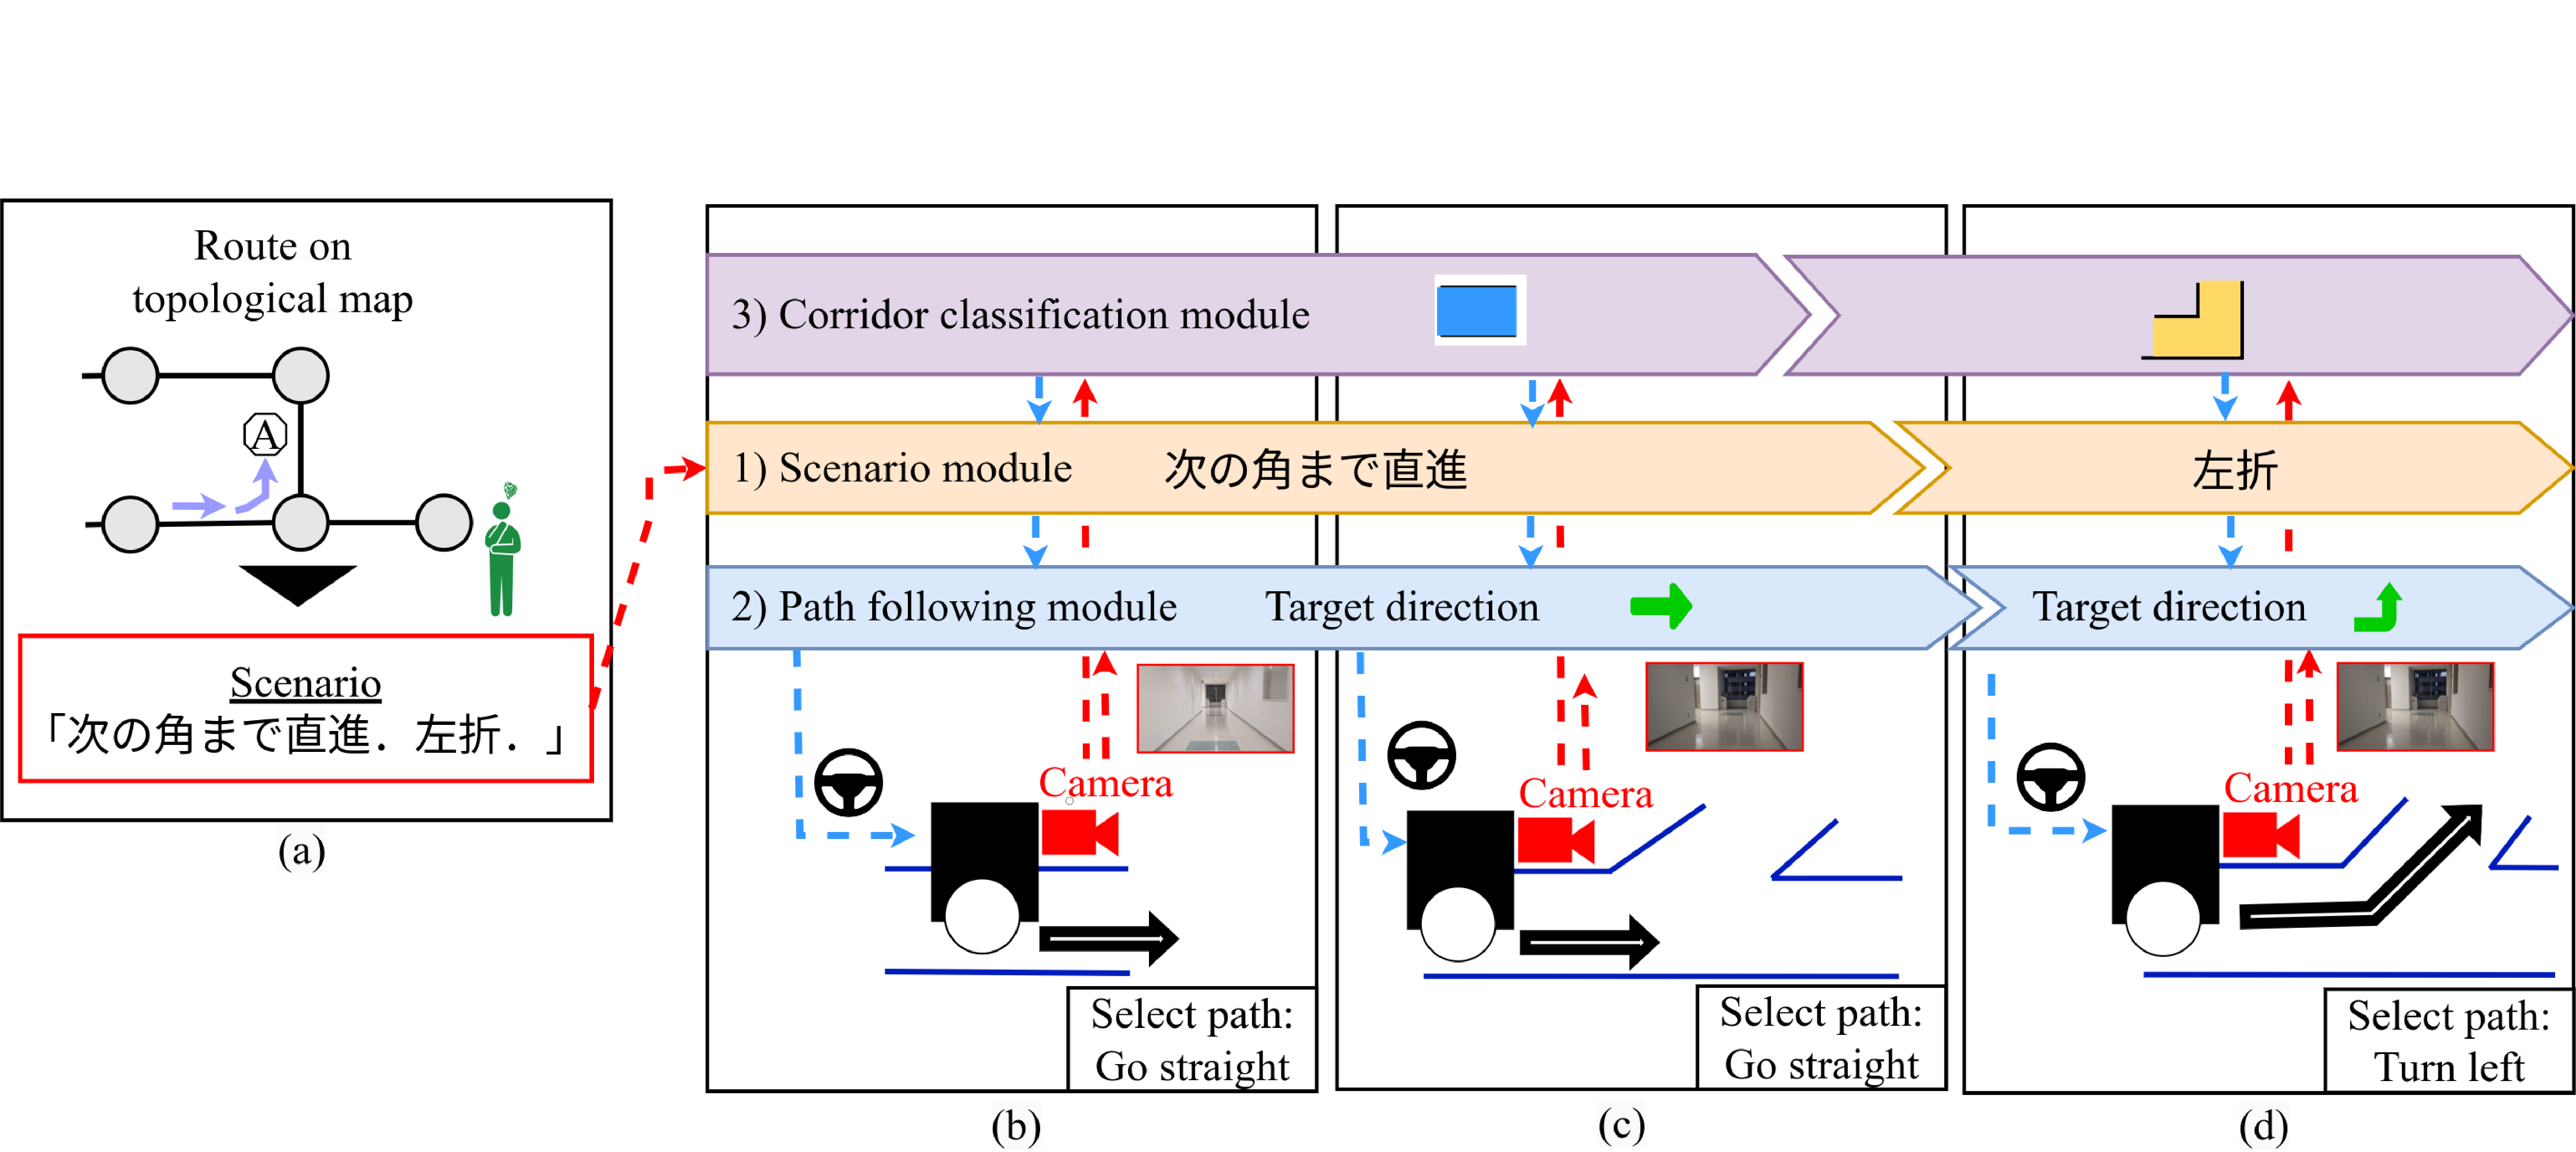
\includegraphics[width=130mm]{images/pdf/absv3.pdf}
     \caption{Overview of constructed system (Quoted from \cite{haruyama2023})}\label{fig:abs}
\end{figure}
\begin{enumerate}
    \item [(a)] トポロジカルマップ上の目的地に応じて,
    人間が「条件」と「行動」で構成されるシナリオを作成する.
    例えば,図のトポロジカルマップ上でAを目的地とするシナリオは「次の角まで直進.左折.」となる.
    \item [(b)] 作成したシナリオをシナリオモジュールへ入力する.
    シナリオモジュールは入力されたシナリオを分解し,「条件」と「行動」を抽出する.
    1つ目の条件と行動のセットは「次の角まで」と「直進」となる.
    この「直進」を目標方向として経路追従モジュールへ与える.
    経路追従モジュールは,カメラ画像と与えられた
    目標方向に基づいて,経路に沿って直進する.
    \item [(c)] ロボットが角に近づくと,
    % 通路分類モジュールの分類結果が角となり,
    通路分類モジュールがカメラ画像に基づいて
    通路を「角」と分類して,それをシナリオモジュールに与える.
    シナリオモジュールはそれを基に「次の角まで」という条件を満たしたかを判定する.
    この場合は条件を満たしているため,2つ目の行動である「左折」
    へ遷移する.
    \item [(d)]「左折」に基づいて,経路追従モジュールは
    経路に沿って角を左折する.
\end{enumerate}

% なお3つのモジュールはRobot Operating System(以下,ROS)\cite{ros}のフレームワーク上で作成している.
% また,通路分類モジュールと経路追従モジュールでは
% 機械学習のフレームワークとしてpytorch\cite{torch}を使用している

\newpage
\section{経路追従モジュール}
\label{sec:imitation}
経路追従モジュールについて述べる.
このモジュールは\ref{chap:path_select}章で述べたシステムに倣って構築した,
カメラ画像に基づいて経路を追従するモジュールであり,
分岐路では入力された目標方向によって経路を選択して走行する.
なお,\ref{chap:path_select}章で述べたシステムに対し,
目標方向とネットワークのパラメータ変更,データセットの収集方法の追加をしている.

% 次に追加した,データセットの収集方法について述べる.
% \ref{chap:path_select}章では,学習器の訓練に60000stepを必要とし,
% 実ロボットを用いた実験に向けて,必要となる学習の量を削減することが望まれる.
% 藤原らが提案する
% データセットに加えるデータの不均衡を改善する手法
% 学習時に積極的に蛇行する手法
% 次に
% \ref{fig:learning_sys}に経路追従モジュールのシステムを示す.


% 学習時は,2D-LiDARやオドメトリ,
% 事前に作成したメトリックマップに基づいた
% ルールベース制御器(ROS Navigation stack)によって,設定した経路を追従する.
% その際,入力をカメラ画像と目標方向,
% 出力をヨー方向の角速度とするデータを,0.2秒周期でデータセットに加える.
% このヨー方向の角速度はメトリックマップに基づいたルールベース制御器が
% 出力する信号である.カメラ画像の収集では
% 中央, 左,右に傾けて取り付けた3つのカメラを用いる.
% 左と右のカメラ画像に対する角速度には,経路に戻るようにオフセットを加える.
% さらに,バッチサイズを8として
% 教師データを抽出し,0.2 秒の周期でオンラインで学習する.
% このデータセットへのデータの追加から学習までの1連の流れを1ステップとする.
% 学習時のデータセットへ加える目標方向には,
% メトリックマップに基づいたルールベースの制御器からの出力を用いる.

% 学習後,モジュールはカメラ画像と目標方向を基に,
% 出力したヨー方向の角速度により経路を追従する.
% このとき,並進速度は 0.2m/s である.
% なお,目標方向が「停止」の場合は,0.0m/s となる.
% \begin{figure}[htbp]
%     \centering
%      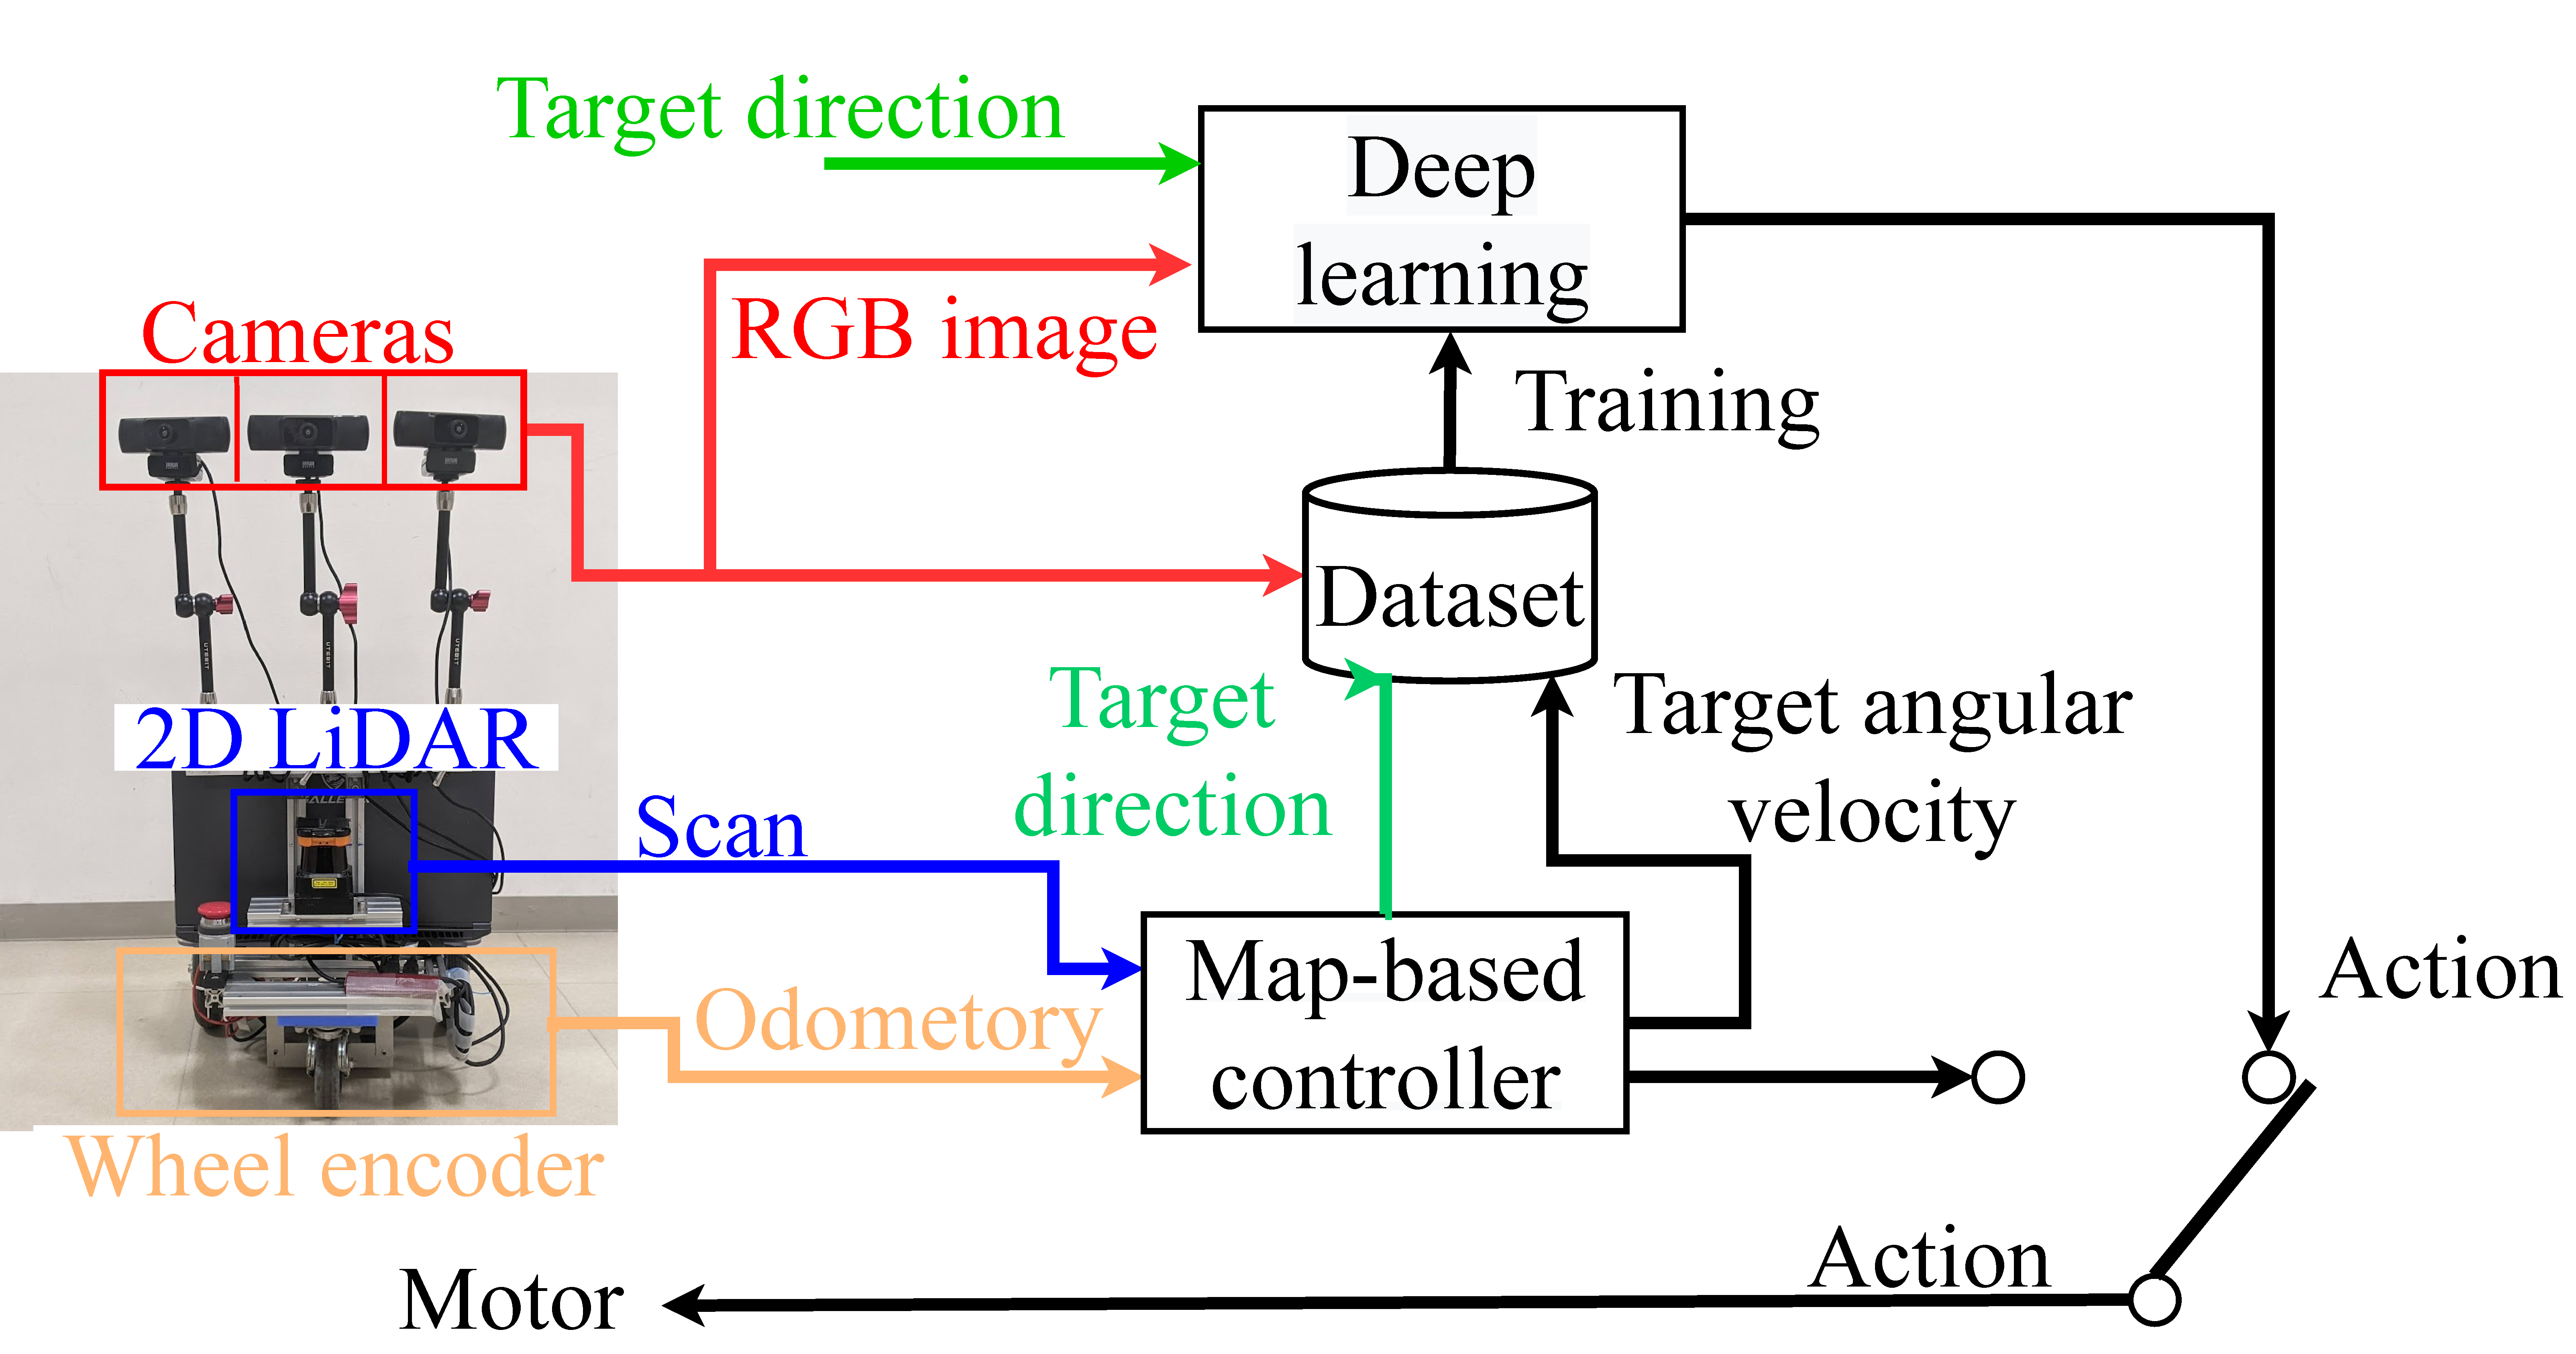
\includegraphics[width=130mm]{images/pdf/system_learning.pdf}
%      \caption{Path-following module system}\label{fig:learning_sys}
% \end{figure}

追加した学習時のデータセットの収集方法は,
% % 岡田ら\cite{okada2021}が提案した
% % \begin{quote}
% %     \begin{itemize}
% %      \item 学習器の出力を監視して,経路追従できない場所のデータのみ選択してデータセ
% %      ットに追加する手法
% %     \end{itemize}
% %    \end{quote}
% の他に
藤原ら\cite{fujiwara2023}が学習量の削減を目的に行った以下の2つの手法である.
\begin{quote}
    \begin{itemize}
     \item データセットに加えるデータの不均衡を改善する手法
     \item 学習時に積極的に蛇行する手法
    \end{itemize}
   \end{quote}


データセットに加えるデータの不均衡を改善する手法について述べる.
\figref{fig:oversmple}に,\chapref{chap:path_select}の実験における10000ステップあたりの目標方向
を青で示す.直進のデータが他に比べ圧倒的に多く,不均衡あることが分かる.
Haiboらの調査\cite{hukinko}では,ほとんどの標準的な学習アルゴリズムは,データの不均衡によりパフォー
マンスが大幅に低下するとされている.
そこで,データ前処理手法であるオーバーサンプリングを用いて,データの偏りを改善する.
具体的には,図中赤で示すように左折と右折を7倍に複製する.
\vspace{3zh}
\begin{figure}[htbp]
    \centering
     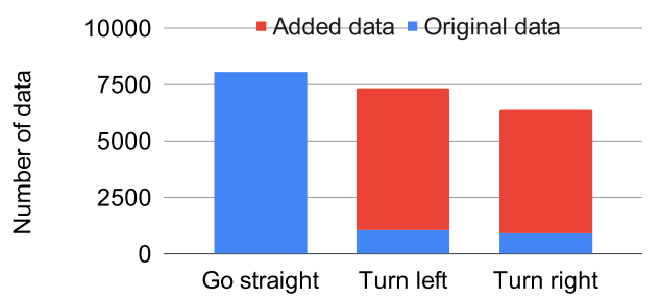
\includegraphics[width=100mm]{images/pdf/oversmple.pdf}
     \caption{Number of data in the target direction per 10000 steps
     in the previous experiment Quote from \cite{fujiwara2023}}\label{fig:oversmple}
\end{figure}
\clearpage
次に,学習時に積極的に蛇行する手法について述べる.
学習時に経路から離れた状態が増加すると,訓練済みの学習器での走行時に経路から
外れることが減少し,より少ない学習時間で成功率が高いモデルができる可能性がある.
そのため,学習時に積極的に蛇行する手法では\figref{fig:dakou}に示すように,
学習時のロボットの制御に用いるヨー方向の角速度を1.5倍にする.
これにより,大きく蛇行して,目標経路から離れた状態を多く収集する.

藤原らは実験により,これらの2つのデータセットの収集手法によって,
経路追従の成功率を下げること無く,必要な学習量を60000ステップから
20000ステップまで削減できることを確認している.
\begin{figure}[htbp]
    \centering
     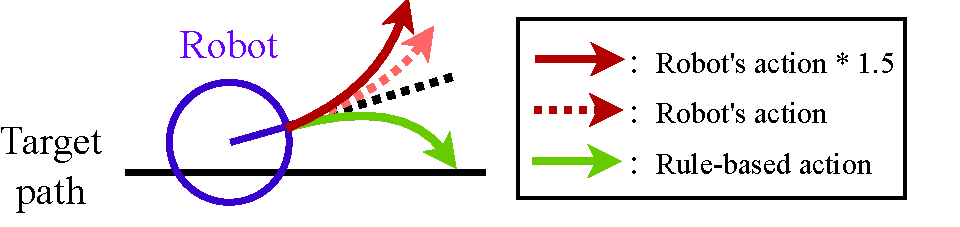
\includegraphics[width=130mm]{images/pdf/dakou.pdf}
     \caption{Aggressive meandering (Quote from \cite{fujiwara2023})}\label{fig:dakou}
\end{figure}
\newpage

\tabref{tab:target}に変更した目標方向とそのデータ形式を示す.
\chapref{chap:path_select}における
目標方向の中で,ContinueとGo straightは同じ方向を指しているため,本章ではこれらを1つとして扱う.
これに伴い,ワンショットベクトルの次元数を4から3へ変更している.
さらに,目的地に到着後,ロボットを停止させることを目的として,
Stop(停止)の目標方向を追加した.
停止の目標方向が入力された際には,ロボットの並進速度は0.0m/sとなり,ロボットはその場で停止する.
% なお,停止以外の目標方向における並進速度は\chapref{chap:path_select}と同様に0.2m/sである.
% 「停止」が入力された場合は0.0m/sとなる.

目標方向の次元数に伴い,変更を加えたネットワークの構造を\figref{fig:imi_net}に示す.
具体的には,CNNの出力と目標方向を入力する全結合層の入力サイズを260から259へ調整している.

\begin{table}[htbp]
    \centering
    \caption{Target direction and data for path-following module}\label{tab:target}
    \begin{tabular}{|c|c|}
    \hline
    Target direction & Data        \\
    \hline
    Go straight   & {[}1,0,0{]} \\
    Turn left   & {[}0,1,0{]} \\
    Turn right   & {[}0,0,1{]} \\
    Stop   & {[}0,0,0{]}\\
    \hline
    \end{tabular}
    \end{table}
% 経路追従モジュールで用いるネットワークの構造を\ref{fig:imi_net}に示す.
% ネットワークはRGB画像と,目標方向を入力,ヨー方向の角速度を出力として
% end-to-endで学習する.
% ネットワークは,画像を処理するCNNアーキテクチャ,
% CNNの出力と目標方向を入力とする全結合層で構成されている.
\begin{figure}[htbp]
    \centering
     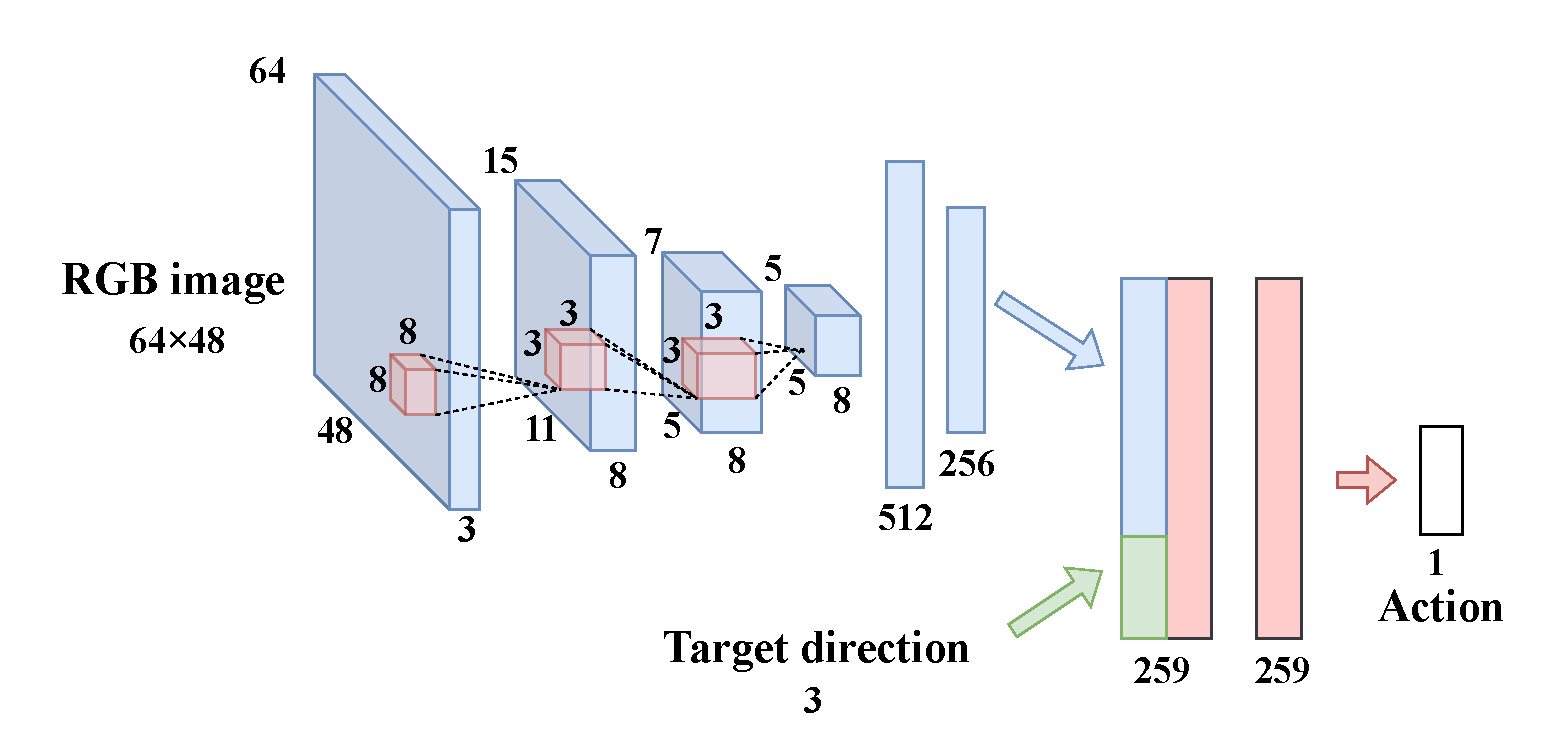
\includegraphics[width=130mm]{images/pdf/imi_net.pdf}
     \caption{Structure of the network of route selection module}
     \label{fig:imi_net}
\end{figure}

% 目標方向は\ref{tab:target}に示す
% 直進,左折,右折の3つをワンホットベクトルとして入力する.
% この中で,停止はネットワークへは入力せず,
% この目標方向が停止の場合には,前述の通り並進速度,角速度ともに0.0m/sとする.

\newpage
\clearpage
\section{通路分類モジュール}
\label{sec:intersection}
通路分類モジュールについて述べる.
このモジュールは,
シナリオの「条件」が満たされたかの判定に必要な
通路の特徴を,カメラ画像を入力として分類する.
通路分類モジュールの概要を\figref{fig:intersection_abs}に示す.
モジュールはフレーム数16,画像サイズ64x48の連続した画像データを入力とし,
通路の特徴を分類した結果を出力する.
通路の特徴の分類は,島田らの手法に倣い,\figref{fig:class}に示す8つとしている.
使用するカメラは,経路追従モジュールと同様に,データセットの収集時は3つ,
学習後は1つである.

% この中で,突き当たりは
% 行き止まり,角(右),角(左),三叉路(中央)
% 右手に通路が〜角(右)十字路 三叉路(右)三叉路(中央)
% 左手に通路が〜角(左)十字路 三叉路(中央)三叉路(左)
\begin{figure}[htbp]
    \centering
     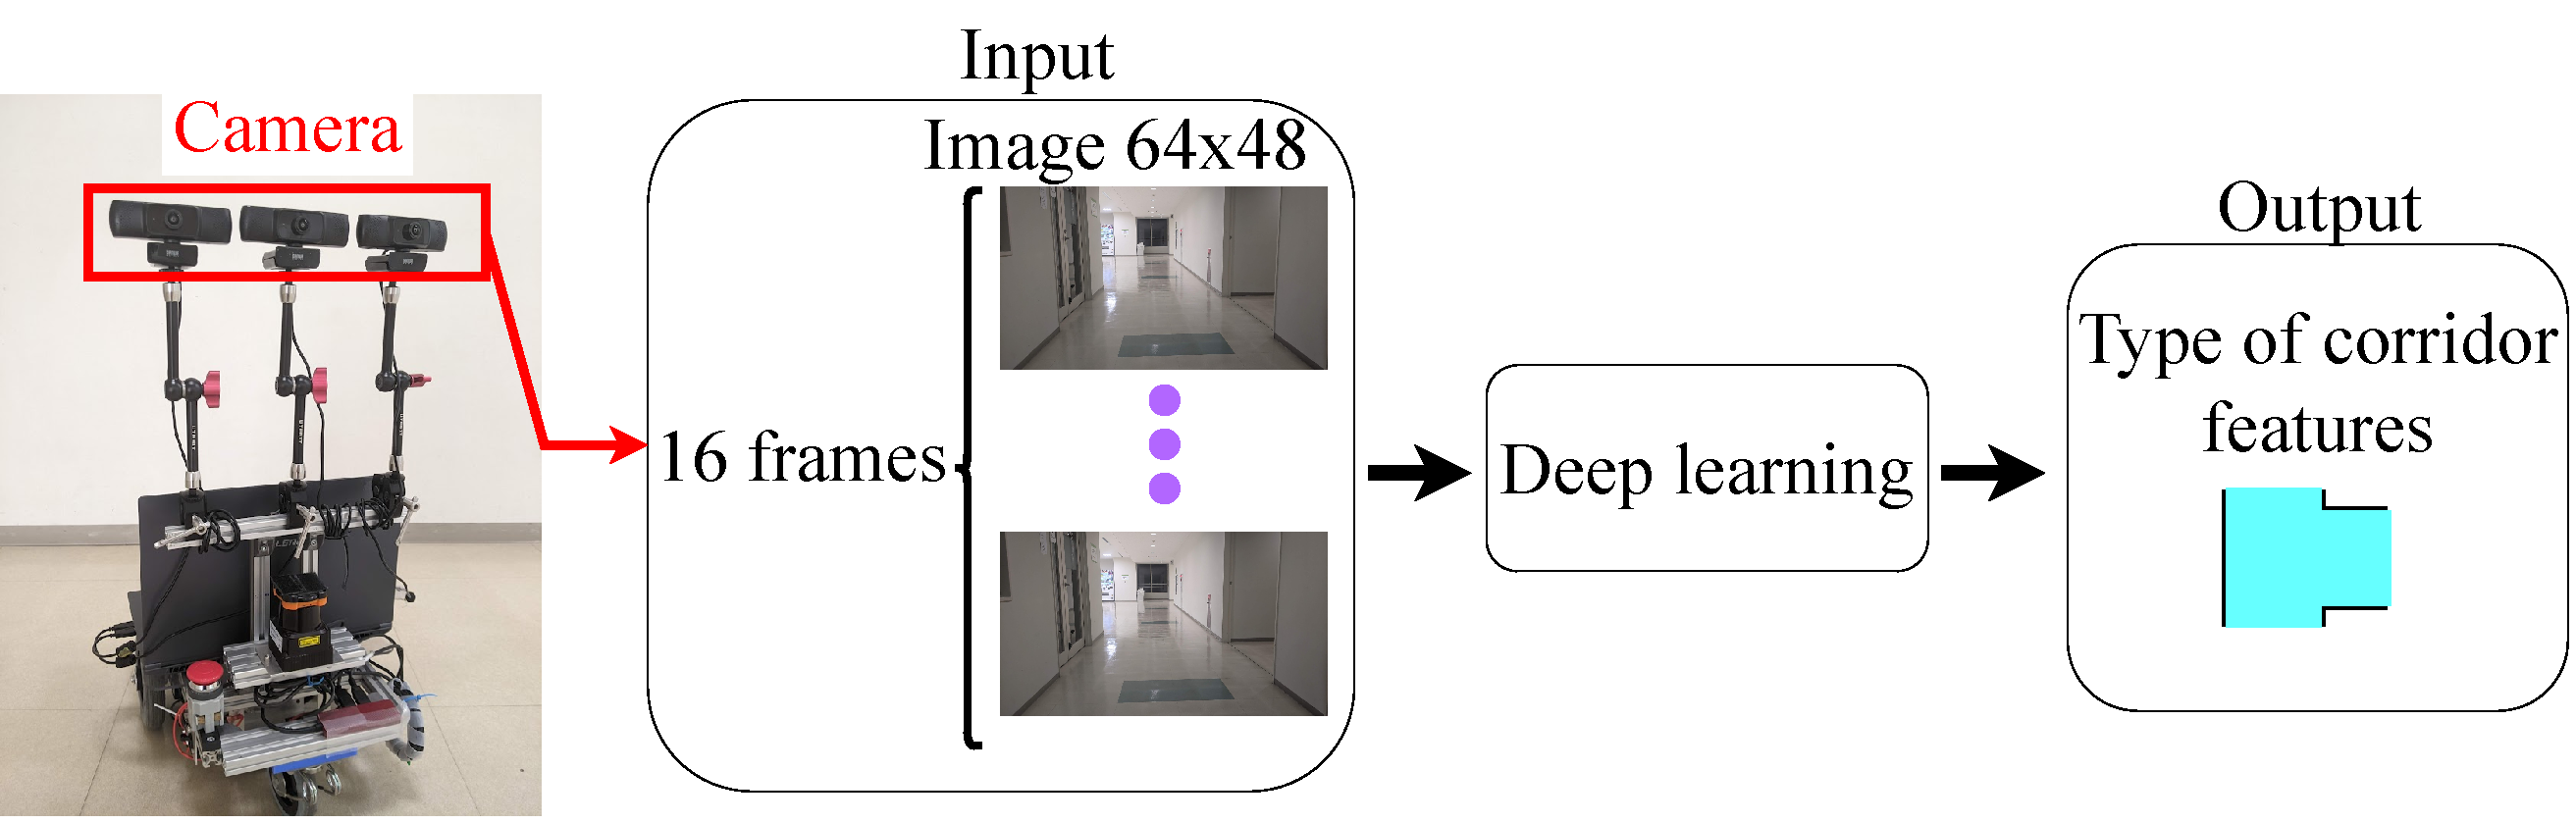
\includegraphics[width=100mm]{images/pdf/intersection_abs.pdf}
     \caption[Overview of the corridor classification module]{Overview of the corridor classification module(Quoted from \cite{haruyama2023})}
     \label{fig:intersection_abs}
\end{figure}
\begin{figure}[htbp]
    \centering
     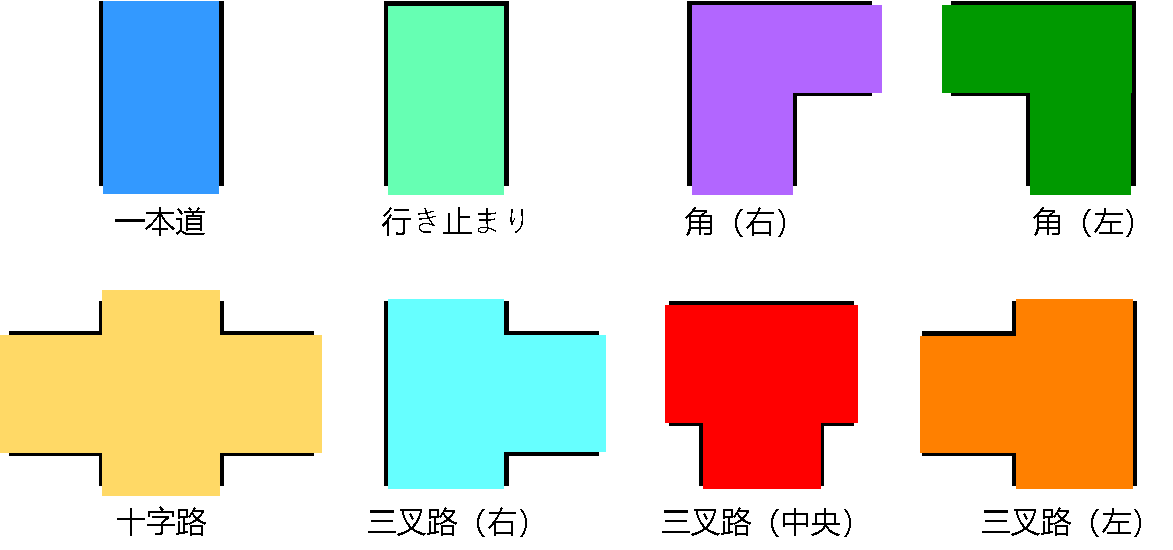
\includegraphics[width=100mm]{images/pdf/class.pdf}
     \caption[Types of corridor features]{Types of corridor features(Quoted from \cite{haruyama2023})}
     \label{fig:class}
\end{figure}
\newpage

ネットワークの構成を\figref{fig:int_net}に示す.
このネットワークアーキテクチャはDhaivatら\cite{lrcn}が提案するCNNとLSTMを組み合わせた
IntersectNetに倣って構築した.
なおCNNアーキテクチャは実時間性の観点からAlexNet\cite{alex}からMobileNetV3-Large\cite{v3}へ変更している.

ネットワークはフレーム数16,画像サイズ64x48の連続したRGB画像データを入力とする.
画像データは各フレームごとにCNNで処理され,この特徴ベクトルはLSTMへ入力される.
各LSTMの出力は分類層(全結合層)へ渡される.
最後に,すべての分類層の出力を融合層へ渡し,融合層は入力の平均を取ることで,
最終的な分類結果を出力する.
活性化関数としてReLU,最適化アルゴリズムにはAdam,損失関数としてCrossEntropyLossを使用する.
\begin{figure}[htbp]
    \centering
     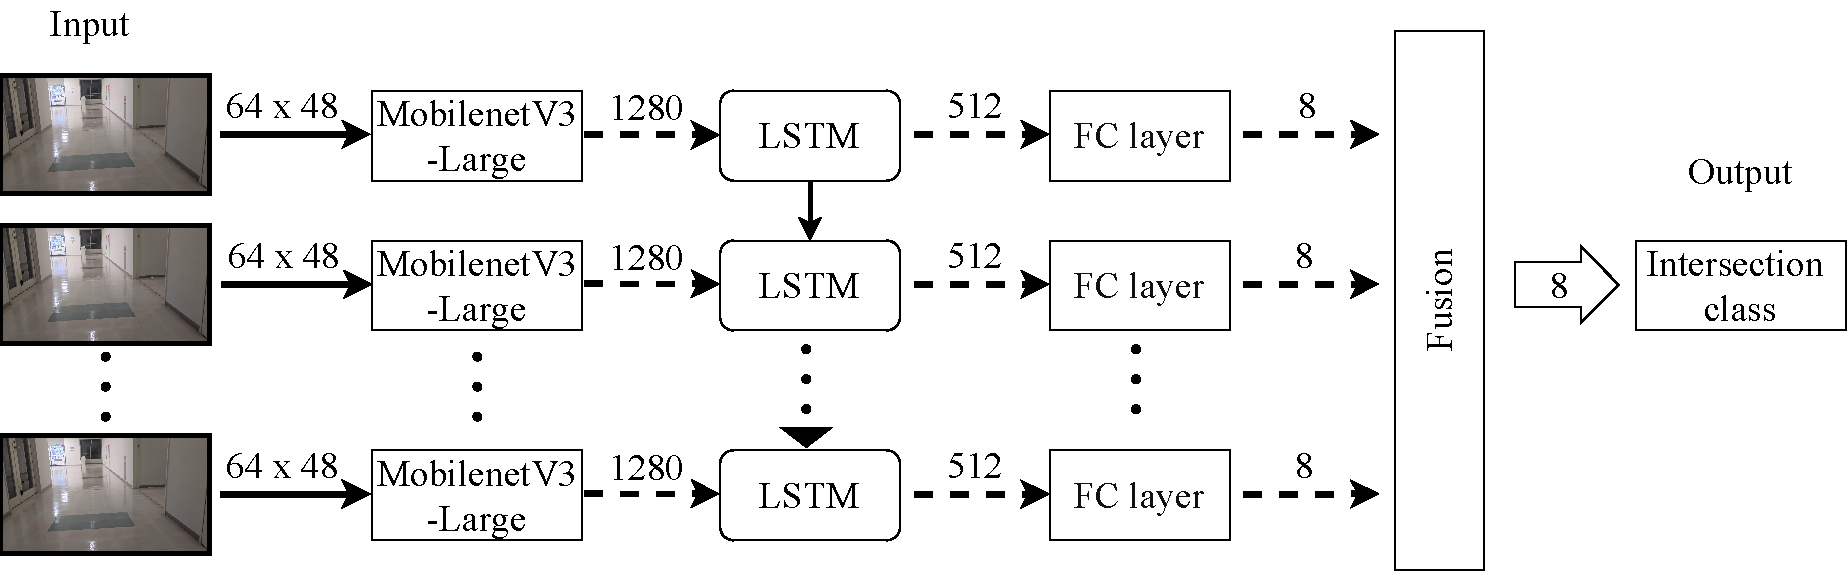
\includegraphics[width=120mm]{images/pdf/network-intersect.pdf}
     \caption{Network of corridor classification module}
     \label{fig:int_net}
\end{figure}

\newpage
次に通路分類モジュールのデータセットの作成について述べる.
データの作成では,経路追従モジュールの学習と同様に,
メトリックマップに基づいたルールベース制御器によって経路を走行する.
その際,フレーム数 16 の連続したカメラ画像と通路の分類ラベルを1組とし,
0.125秒周期でデータセットへ加える.分類ラベルのアノテーションは,
\figref{fig:int_net}に示すように,通路の特徴を予めメトリックマップに登録しておくことで,自動的に行う.
\begin{figure}[htbp]
    \centering
     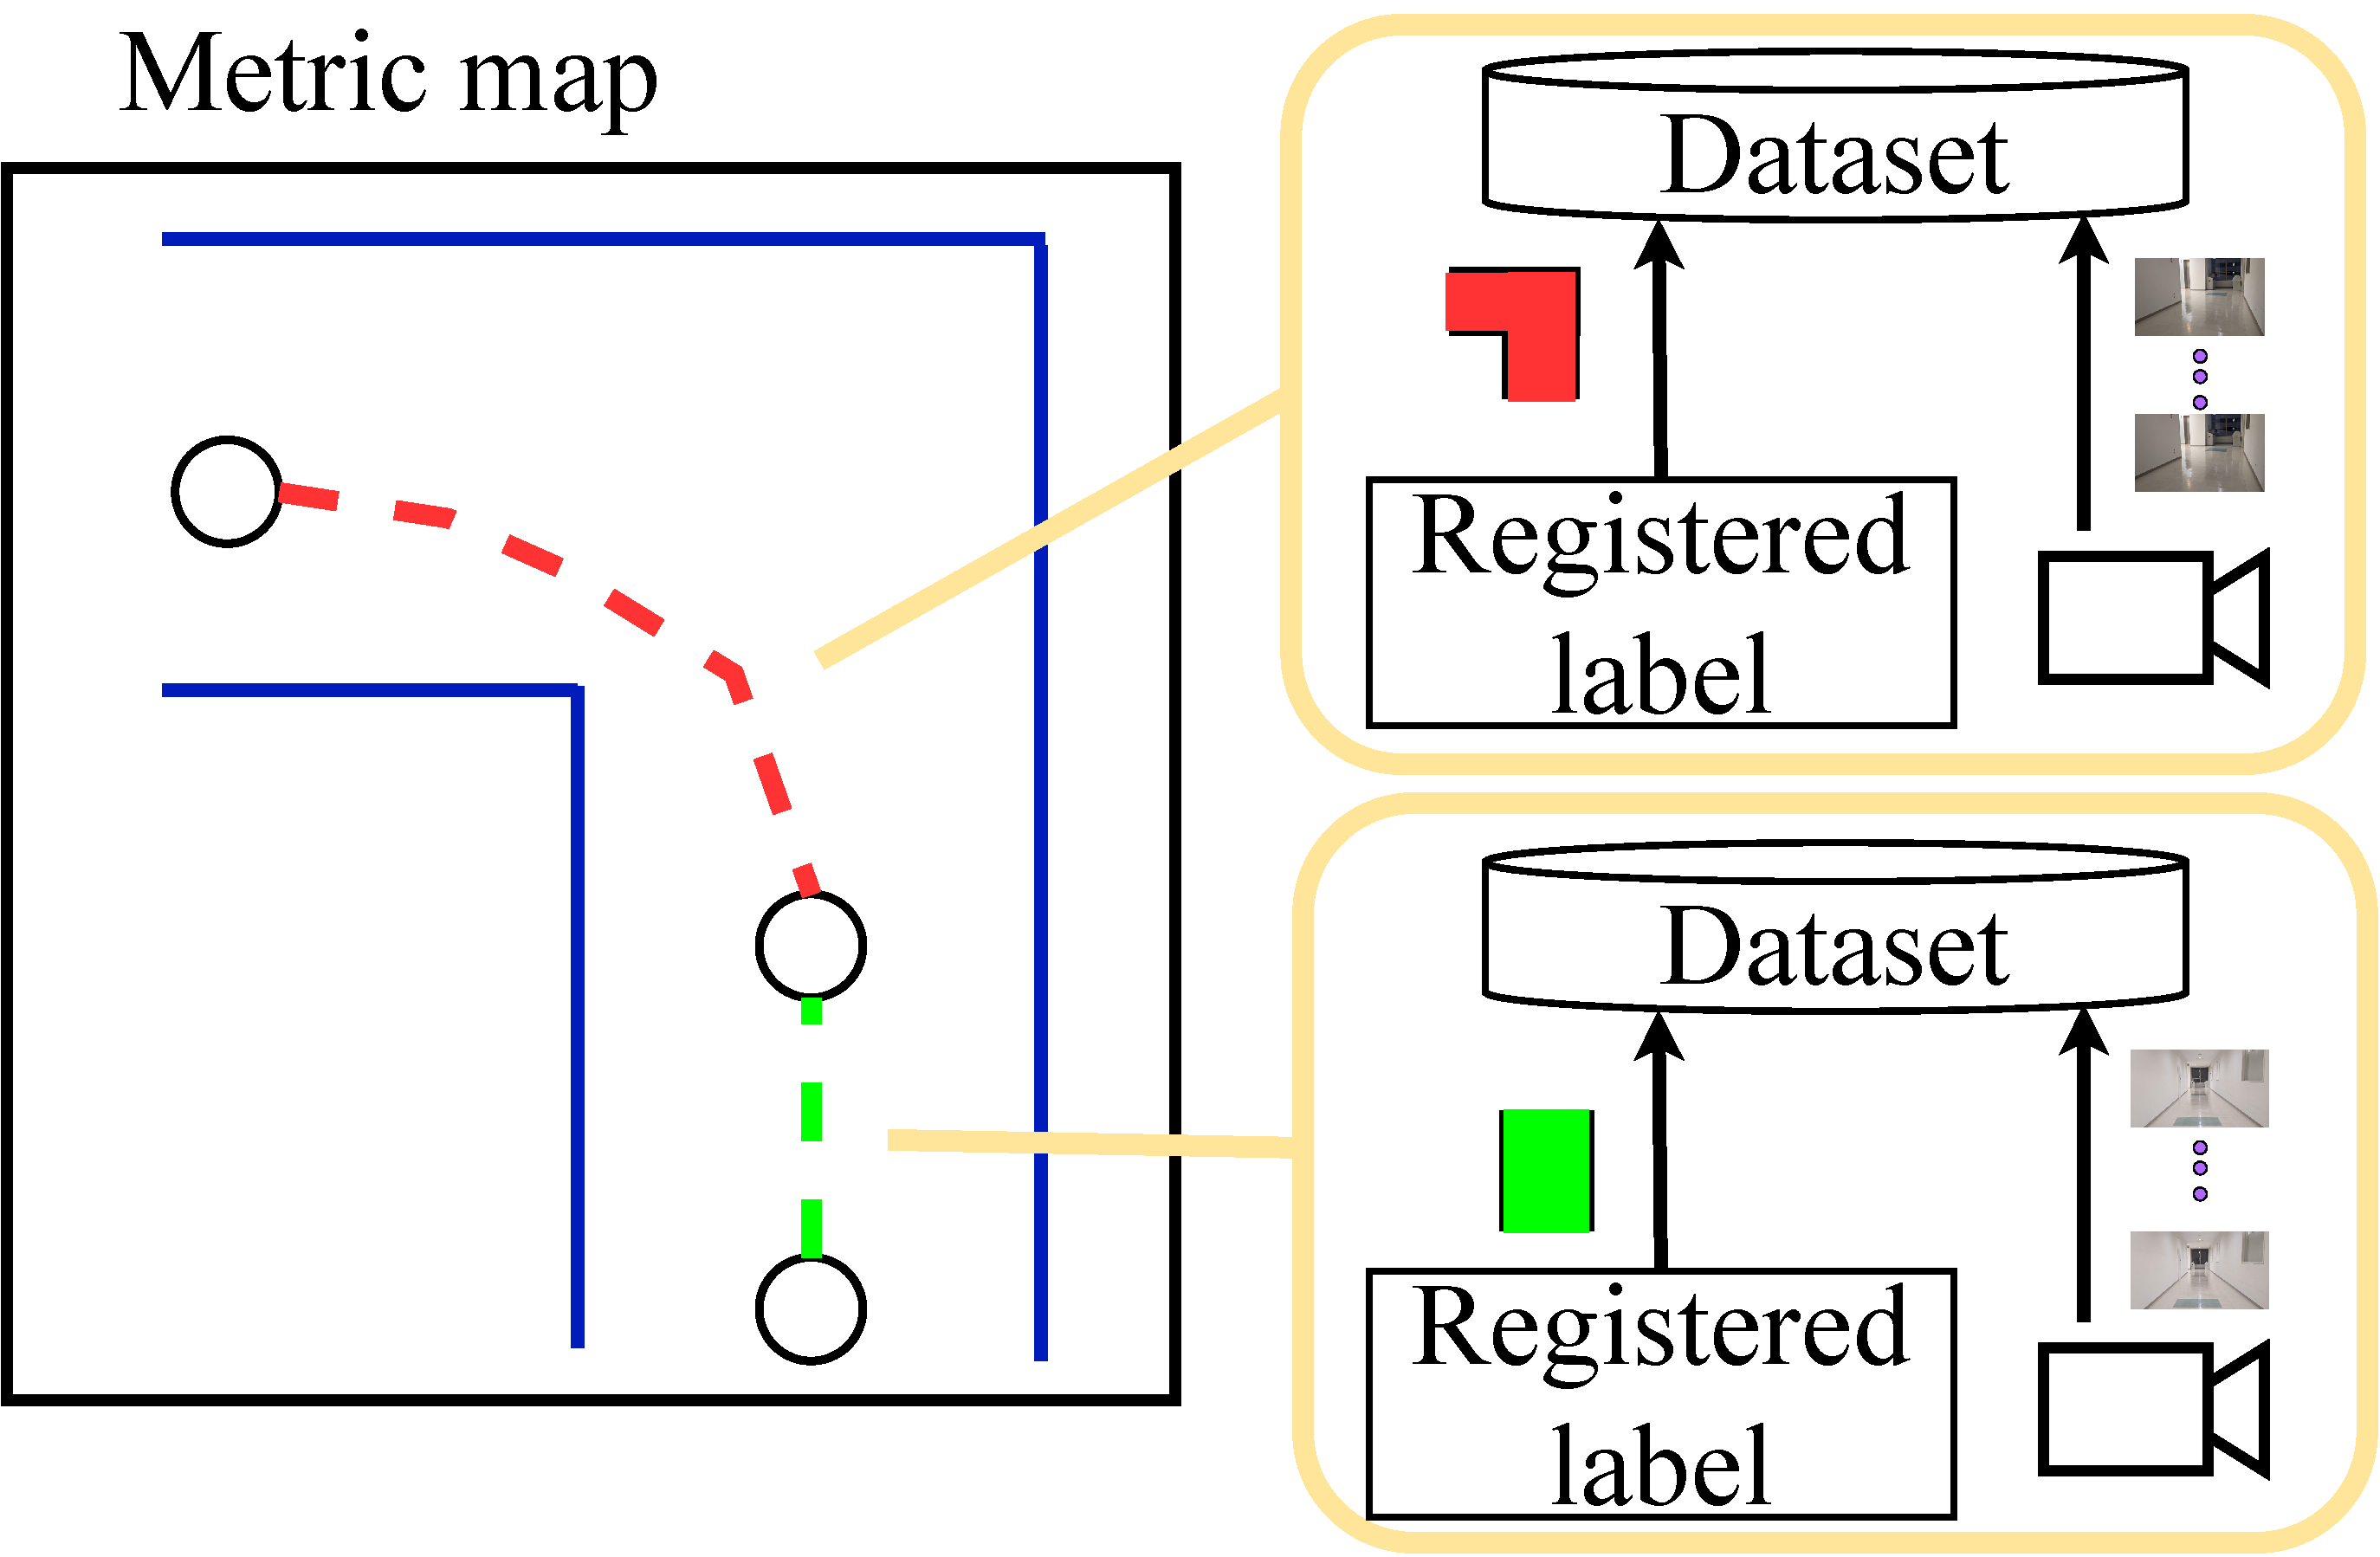
\includegraphics[width=100mm]{images/pdf/map_label.pdf}
     \caption[Classification labels registered in the metric map]{Classification labels registered in the metric map(Quoted from \cite{haruyama2023})}
     \label{fig:int_net}
\end{figure}

\secref{sec:imitation}では不均衡データへの対策として,オーバーサンプリングを行った.
この通路文類モジュールでは,不均衡データへの対策として,
データセット内のクラス間のデータ数によって重み付けを行うコストアプローチ\cite{cost}を行う.
具体的には,損失関数(CrossEntropyLoss)で用いるクラスごとの重みをデータ数を基に調整する.
\newpage
\section{シナリオモジュール}
\label{sec:scenario}
シナリオモジュールについて述べる.
シナリオモジュールはトポロジカルマップから作成されたシナリ
オから「突き当りまで」という「条件」や「左折」なとの「行動」を解釈し,
単語で構成された経路を分岐路での目標方向へ変換して出力する.

\figref{fig:topo2sce}にトポロジカルマップとそれをもとに作成されるシナリオを示す.
図の例では出発地点をエッジ2,目的地をノード2として,その間のエッジとノードを移動する.
エッジ2からノード1は「三叉路まで」という条件と「直進」という行動,
ノード1からエッジ1は「右折」という行動,
エッジ1からノード2は「突き当り(三叉路)まで」という条件と「直進」の行動で表現される.
これらを統合すると,
最終的に「三叉路まで直進.右折.突き当たりまで直進.停止.」
のシナリオが作成される.

次に作成したシナリオを目標方向に変換する処理を述べる.
はじめにシナリオを句点ごとに分解し,部分シナリオというものを作成する.
この部分シナリオには,次の部分シナリオに遷移するための「条件」とロボットが行う必要がある「行動」
が含まれている.
この部分シナリオを形態素分析(MeCab\cite{2004ConditionalRF})を用いて単語へ分割する.
分割した単語は,「条件」と「行動」を示す以下の項目に分けて登録される.
\begin{enumerate}
    \item [1)] 通路の特徴 例えば,「三叉路」「角」など
    \item [2)] 順番 例えば,「3 つ目の」「2 番目の」など 
    \item [3)] 方向 例えば,「左手に」「右手に」など
    \item [4)] 行動 例えば,「右折」「停止」など
\end{enumerate}
先に示した例は句点ごとに,
三叉路まで直進/ 
右折/   
突き当たりまで直進/  
停止/ 
と分解される.

1つ目の条件と行動は 
1)通路の特徴 三叉路,4)行動 直進,

2つ目の行動は 4)行動 右折となる.

3つ目の条件と行動は
1)通路の特徴 突き当たり 4)行動 直進

4つ目の行動は
4)停止となる.

この4)行動を\tabref{tab:target}で示したデータ形式で表現し,分岐路での目標方向として,経路追従モジュールへ与える.
ここで,「三叉路まで」といった条件を達成したかの判定は,
\secref{sec:intersection}の通路分類モジュールの分類結果を用いて行う.
\vspace{3zh}
\begin{figure}[htbp]
    \centering
     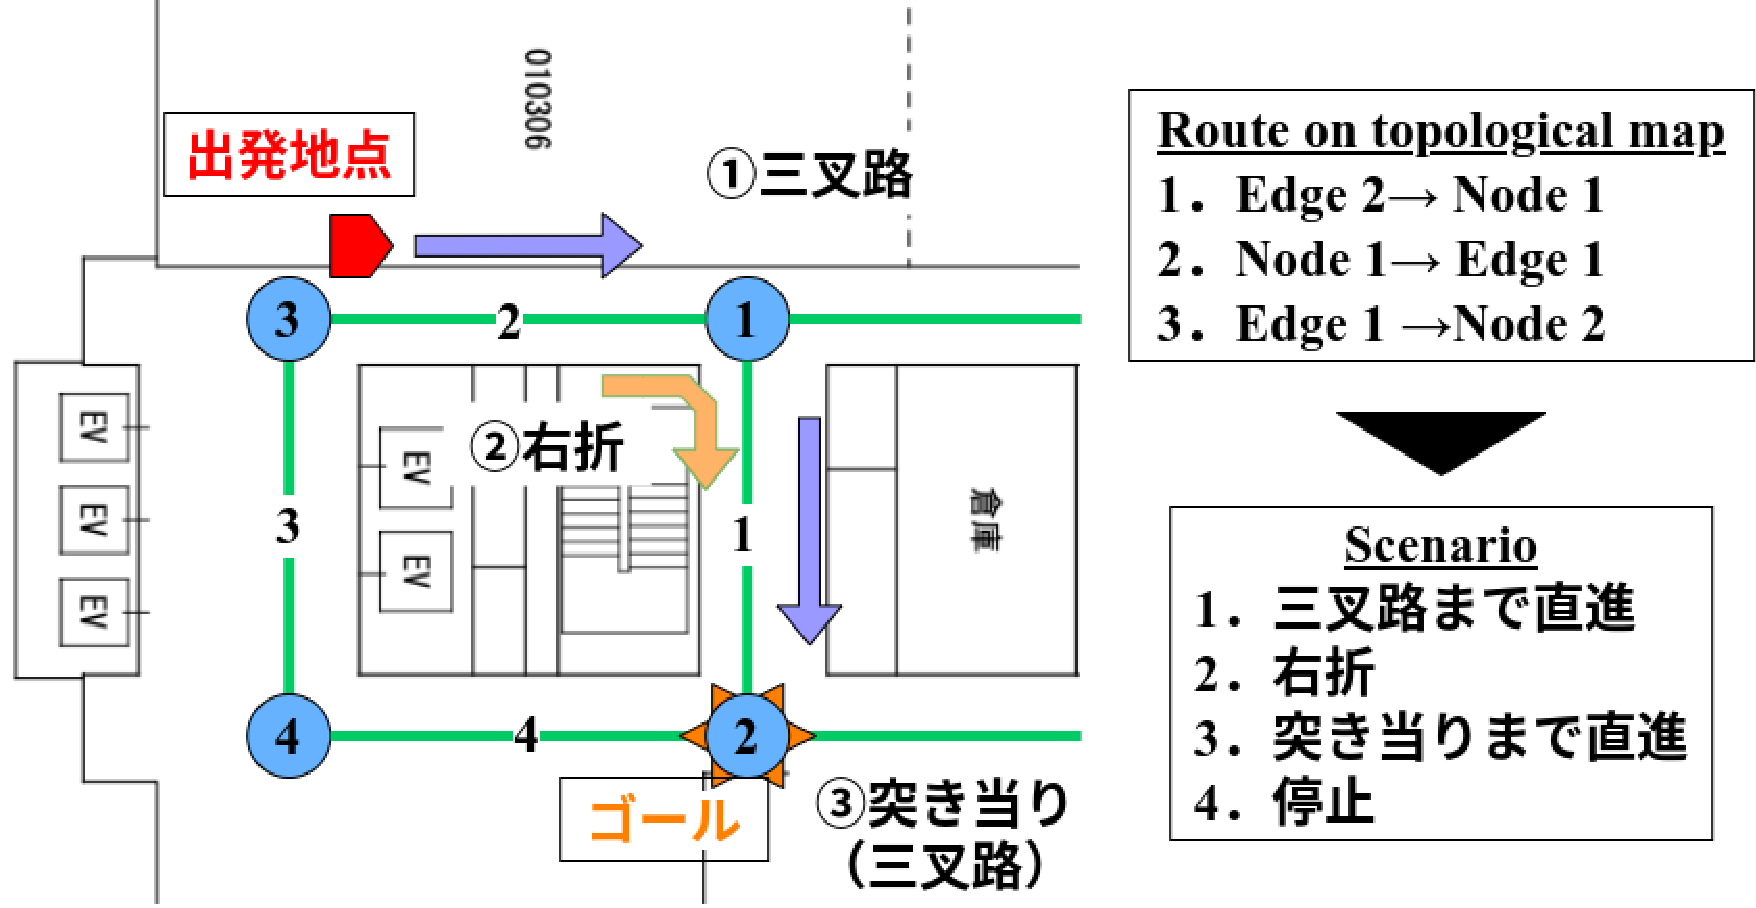
\includegraphics[width=90mm]{images/pdf/topo2sce.pdf}
     \caption[Example of topological map and created scenario]{Example of topological map and created scenario(Quoted from \cite{haruyama2023})}
     \label{fig:topo2sce}
\end{figure}
\newpage
\section{実ロボットを用いた実験}
実ロボットを用いて, 構築したシステムにより, 
ロボットが目的地へ到達可能であるか検証する.
\subsection{実験装置}
実験で用いるロボットを\figref{fig:gamma}に示す.
ロボットはicart-mini\cite{icart}をベースに開発したロボットを用いる.
センサとして,単眼のウェブカメラ(サンワサプライ株式会社 CMS-V43BK)を3つ,
2D-LiDAR(北陽電機 UTM-30LX)を1つ,左右のモータにそれぞれパルス付きエンコーダを搭載している.
制御用の PC には GALLERIA GCR2070RGF-QC-Gを使用している.
メトリックマップに基づくルールベース制御器には,本学でROS Navigation stackをもとに開発した
orne\_navigation\cite{orne_nav}を使用する
\begin{figure}[htbp]
    \centering
     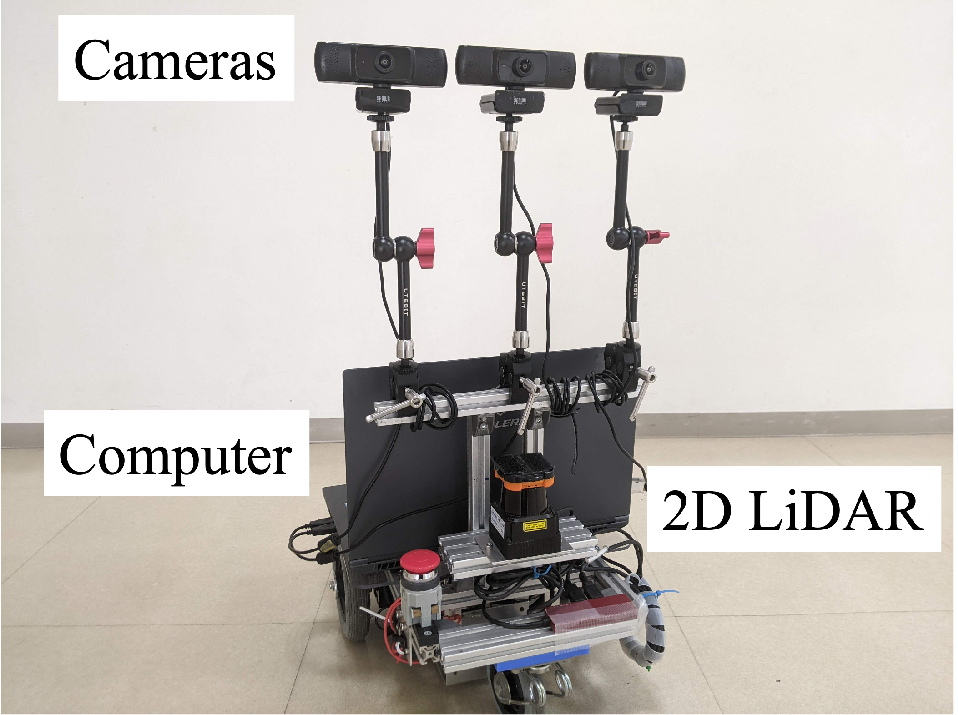
\includegraphics[width=80mm]{images/pdf/gamma_sensor.pdf}
     \caption{Experimental setup (Quoted from \cite{haruyama2023})}\label{fig:gamma}
\end{figure}

\newpage
\subsection{実験方法}
実験環境として\figref{fig:cit3f}に示す千葉工業大学津田沼キャンパス2号館3階の廊下を用いる.
環境中には,三叉路が4つ,角が2つ,突き当たりが2つ含まれている.
経路追従モジュールの訓練および通路分類モジュールのデータセット収集では,
\figref{fig:newroute}で示すaからnの経路を順番に走行する.
\begin{figure}[htbp]
    \centering
     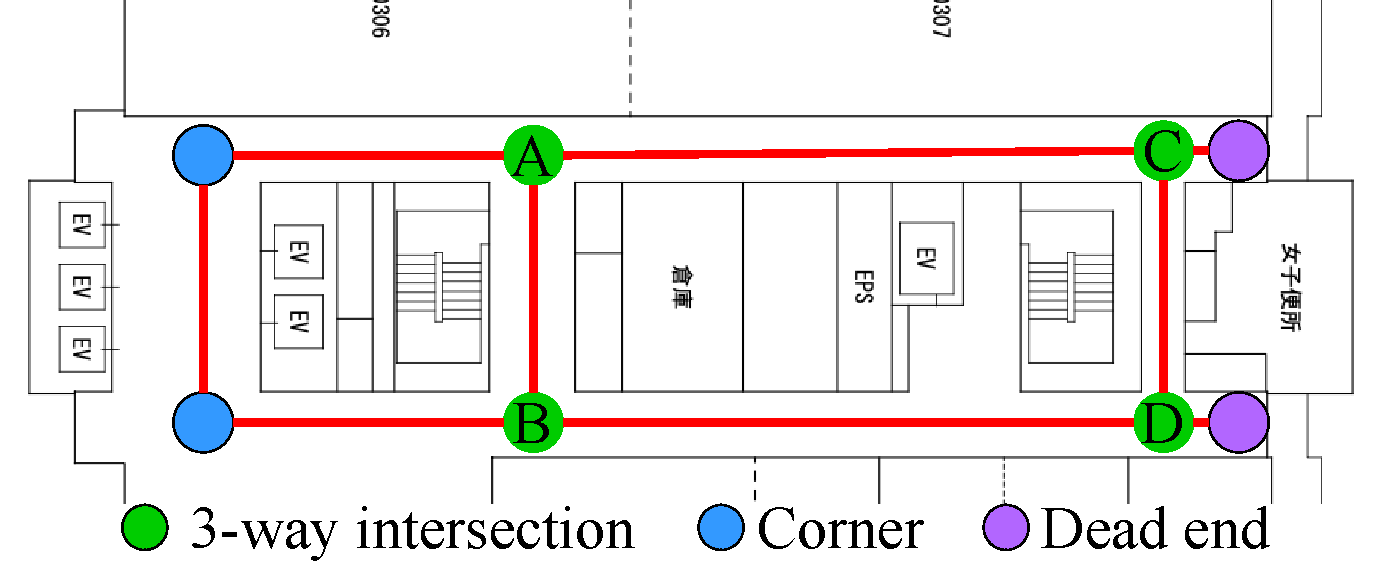
\includegraphics[width=100mm]{images/pdf/cit3f.pdf}
     \caption{Experimental environment (Quoted from \cite{haruyama2023})}\label{fig:cit3f}
\end{figure}
\begin{figure}[htbp]
    \centering
     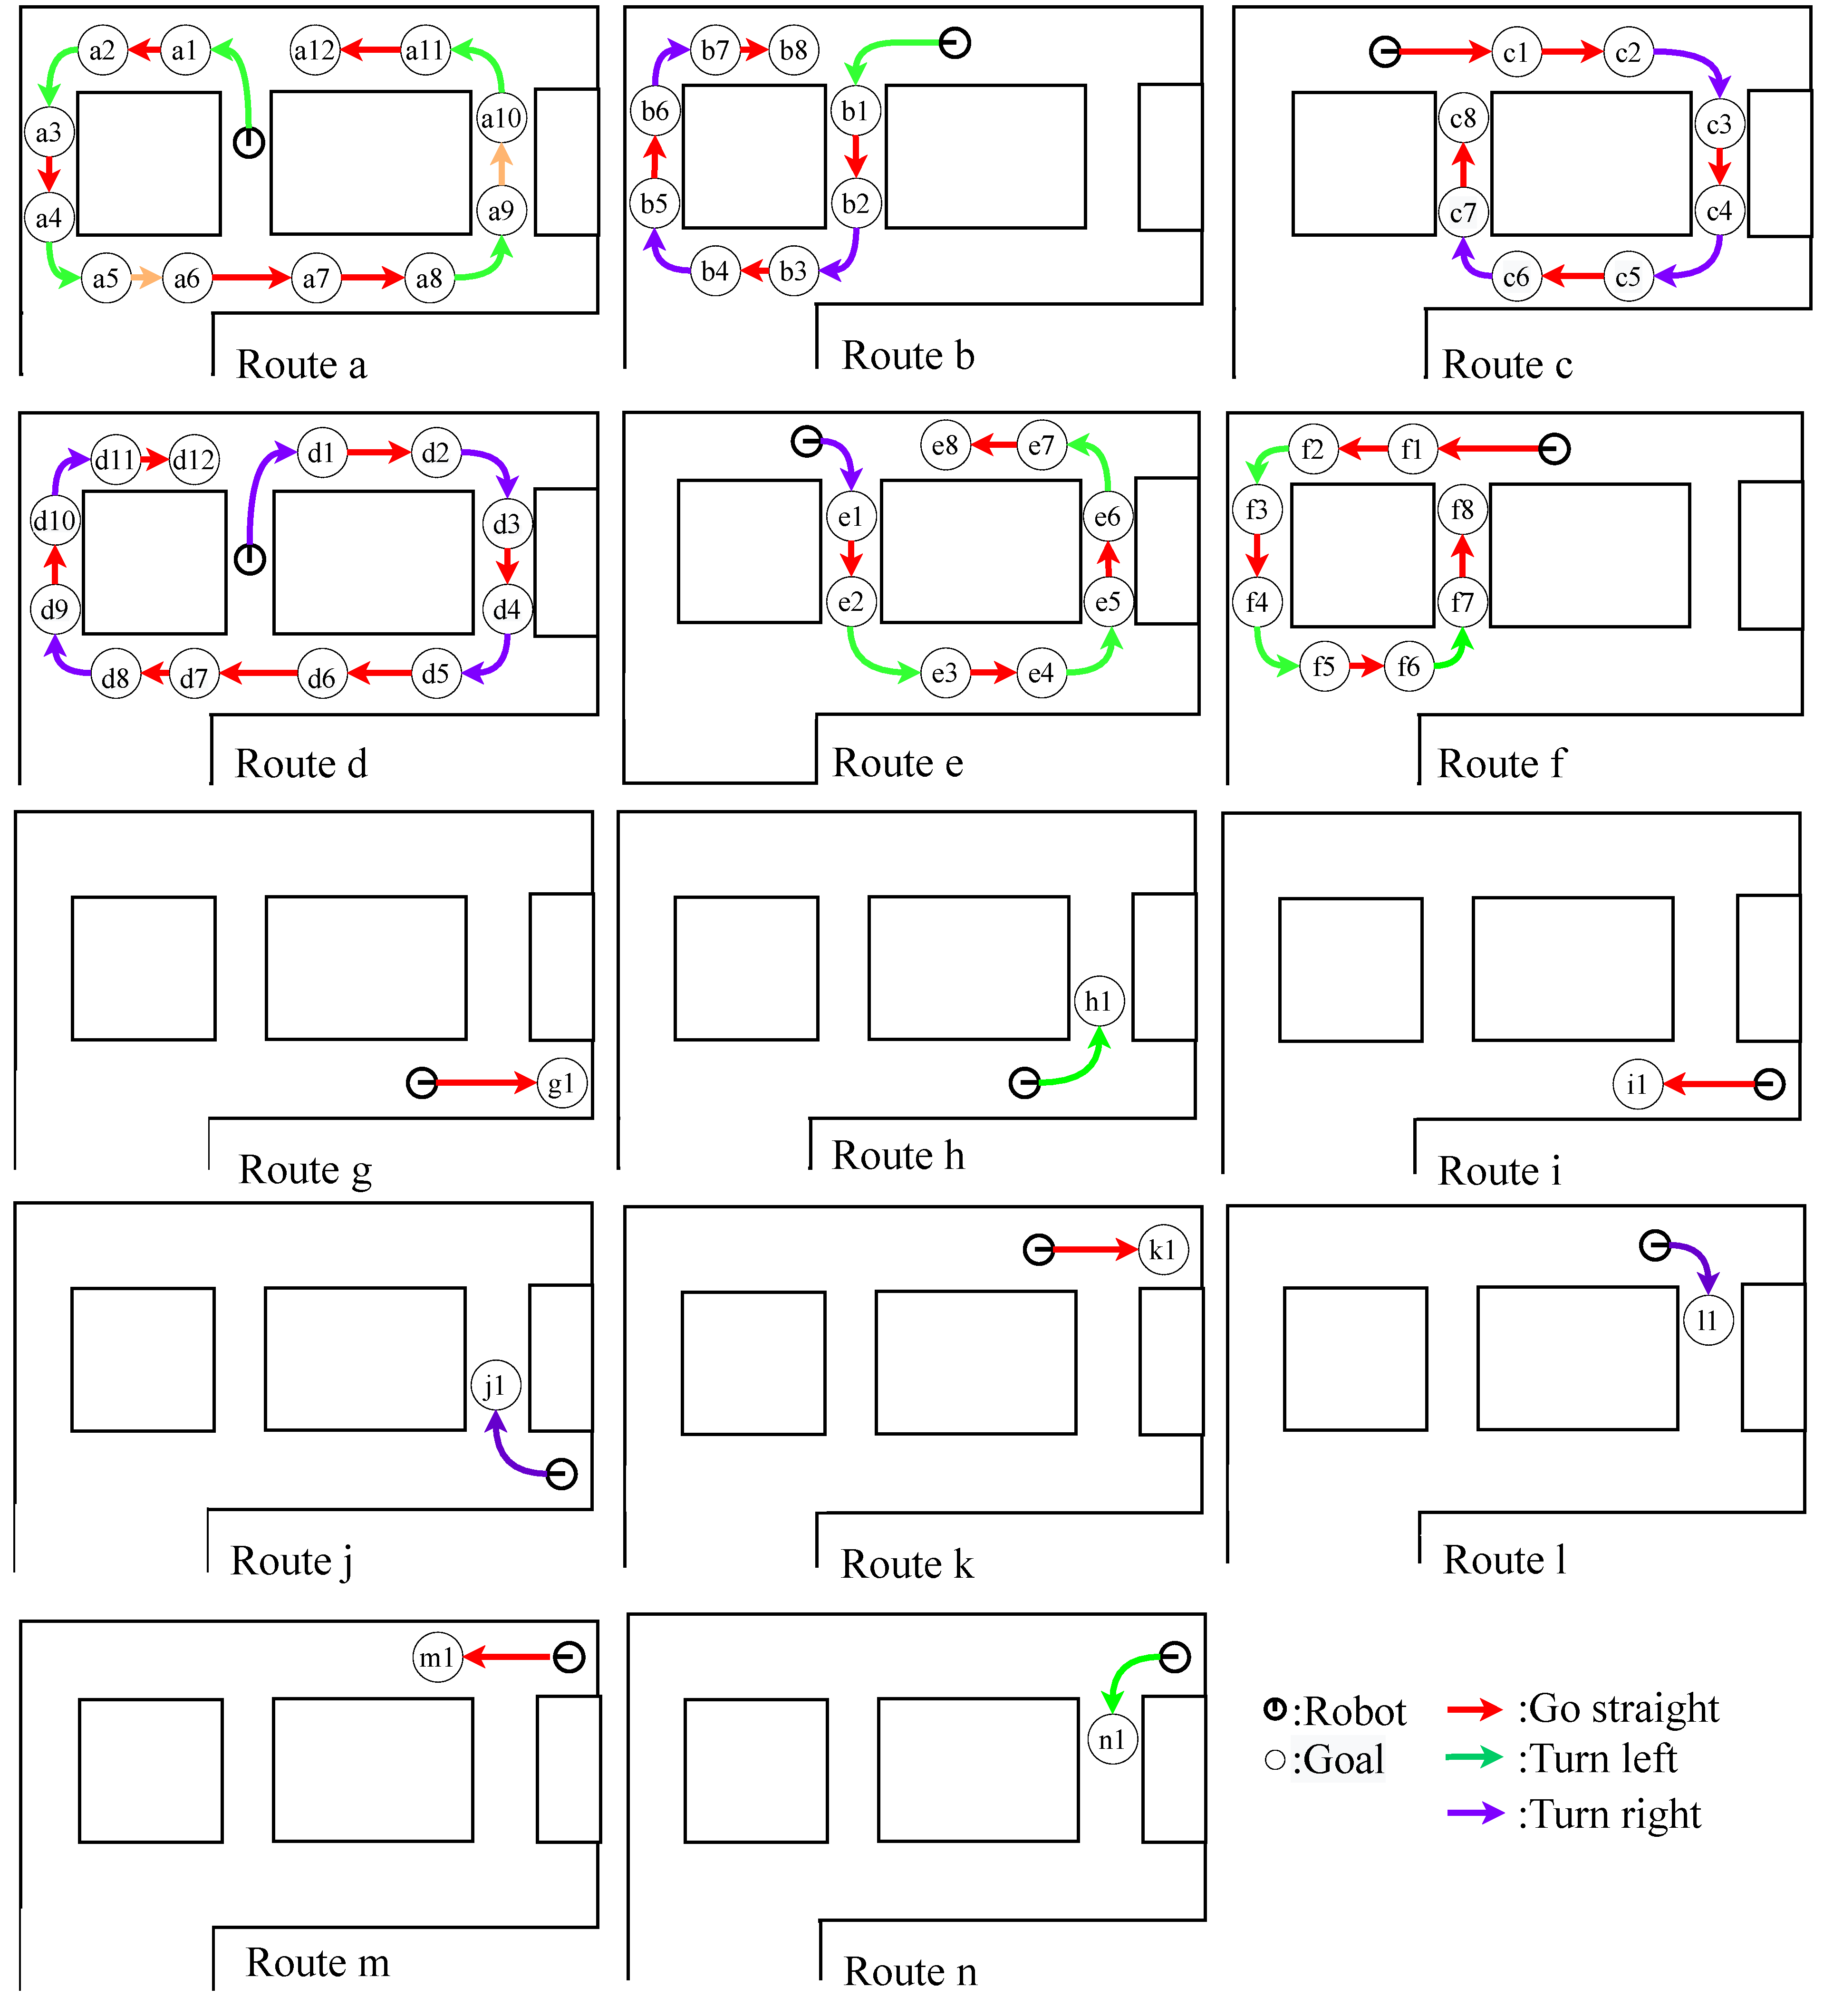
\includegraphics[width=130mm]{images/pdf/si_route.pdf}
     \caption{Route used for learning (Quoted from \cite{haruyama2023})}\label{fig:newroute}
\end{figure}


\subsubsection{シナリオの選定}
実験では島田らが用いた50例のシナリオの中から,
\figref{fig:scenario_exp}に示す7例を用いた.
このシナリオは以下の3つの基準に従って,選定した.
% \ref{fig:cit3f}の場所を対象としていること.
% ロボットが移動困難な\ref{fig:semai}の箇所のような狭い通路が含まれていないこと.
% その場で「後ろを向く」など経路追従モジュールができない行動が含まれていないことである.
\begin{enumerate}
    \item [1)] 2号館3階の廊下において,\figref{fig:cit3f}の場所を対象としていること.
    \item [2)] ロボットが移動困難な\figref{fig:semai}の箇所のような狭い通路が含まれていないこと
    \item [3)] その場で「後ろを向く」など経路追従モジュールができない行動が含まれていないこと
\end{enumerate}

\begin{figure*}[htbp]
    \begin{tabular}{ccc}
        \begin{minipage}[t]{0.5\textwidth}
            \centering
            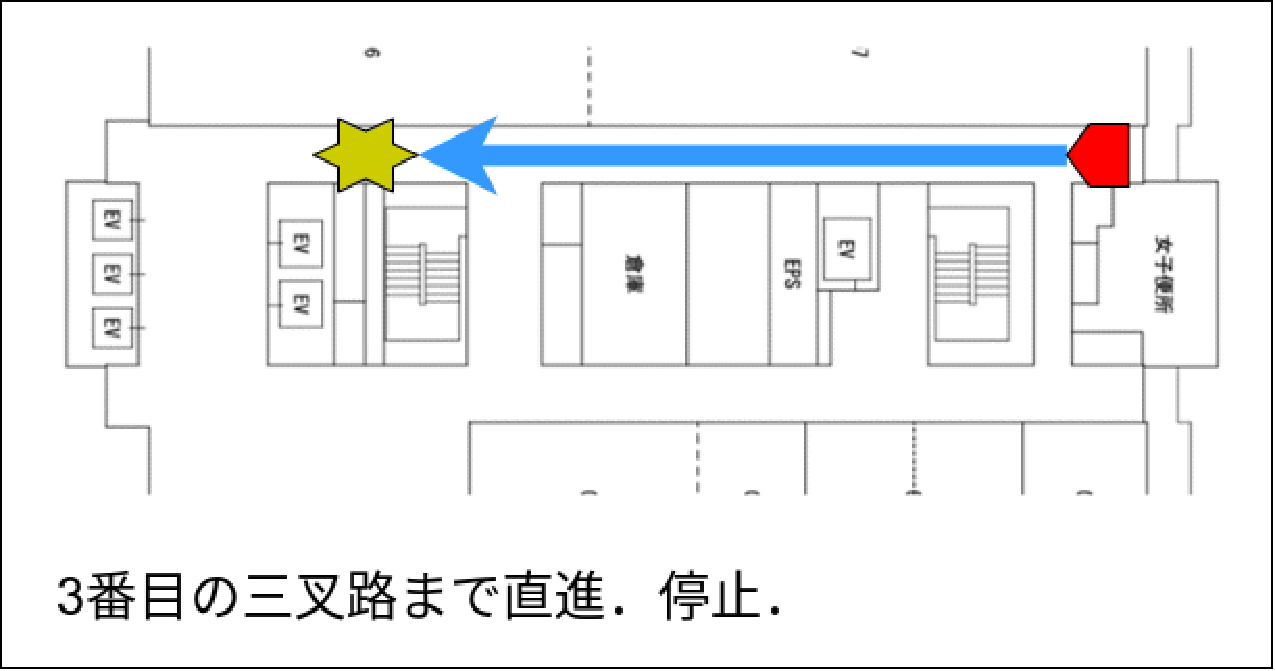
\includegraphics[keepaspectratio, width=57mm]{images/pdf/scenario/scenario01.pdf}
            \subcaption{Scenario 01}
            \label{composite}
        \end{minipage} &
        \begin{minipage}[t]{0.5\textwidth}
            \centering
            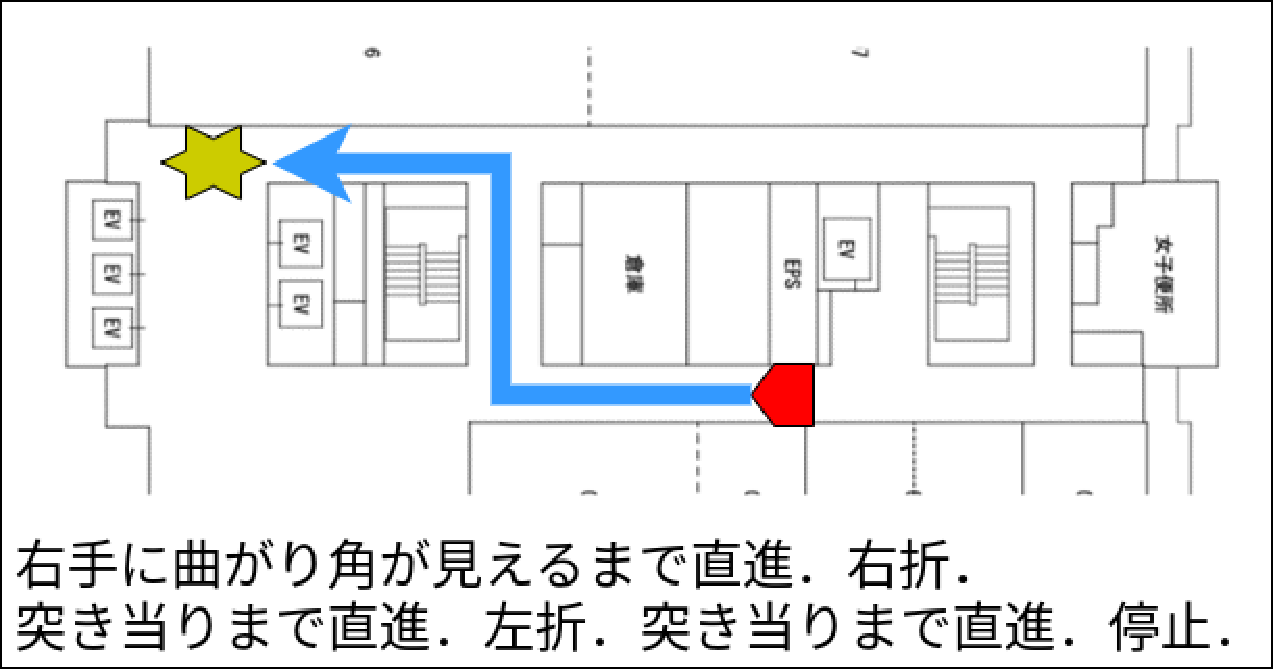
\includegraphics[keepaspectratio, width=57mm]{images/pdf/scenario/scenario02.pdf}
            \subcaption{Scenario 02}
            \label{Gradation}
        \end{minipage} \\
        \begin{minipage}[t]{0.5\textwidth}
            \centering
            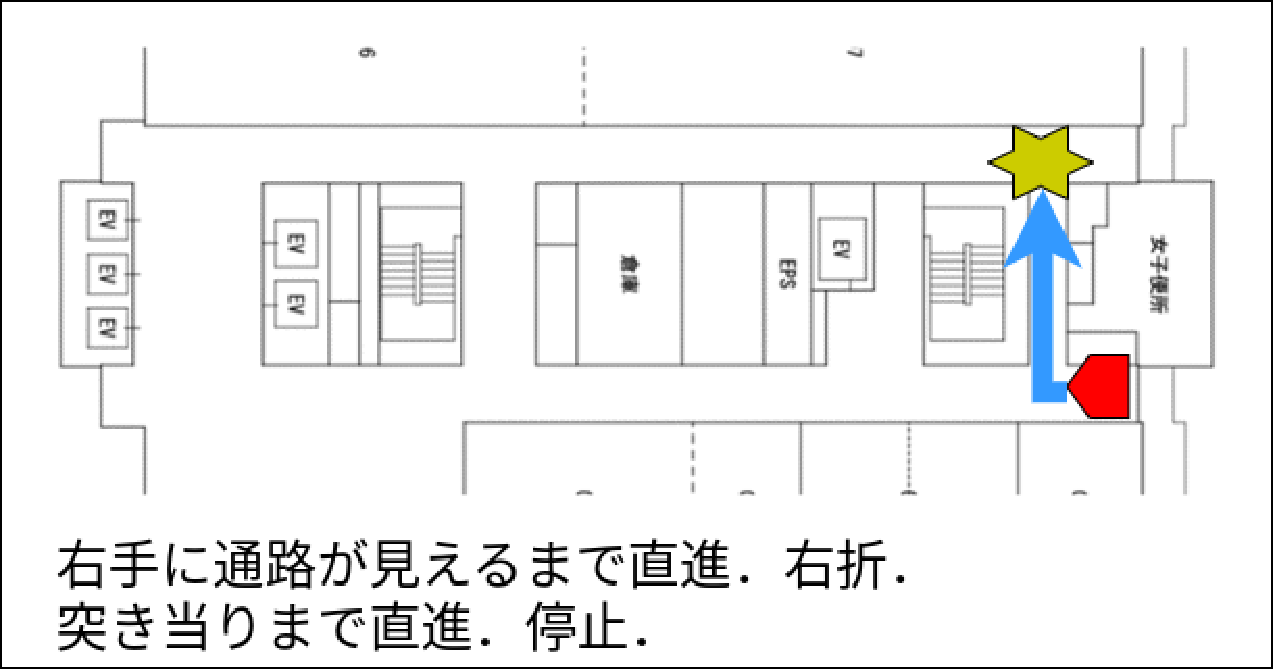
\includegraphics[keepaspectratio, width=57mm]{images/pdf/scenario/scenario03.pdf}
            \subcaption{Scenario 03}
            \label{fill}
        \end{minipage} &
        \begin{minipage}[t]{0.5\textwidth}
            \centering
            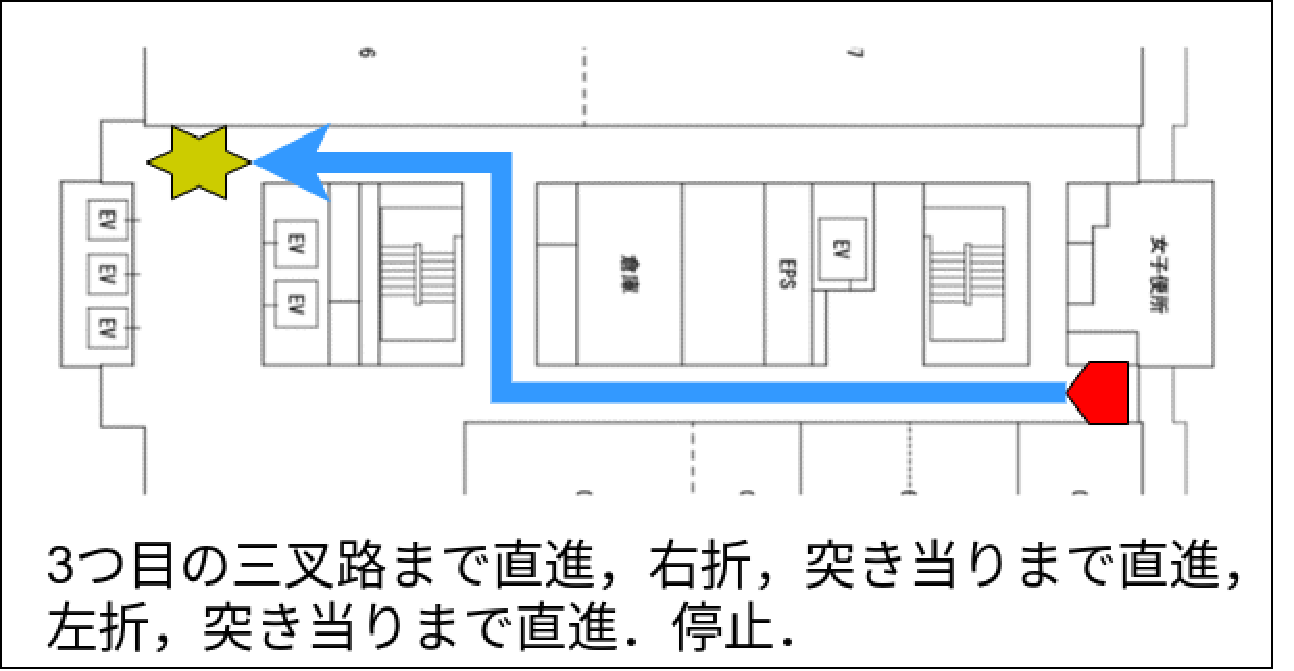
\includegraphics[keepaspectratio, width=57mm]{images/pdf/scenario/scenario04.pdf}
            \subcaption{Scenario 04}
            \label{fig:scenario21}
        \end{minipage} \\
        \begin{minipage}[t]{0.5\textwidth}
            \centering
            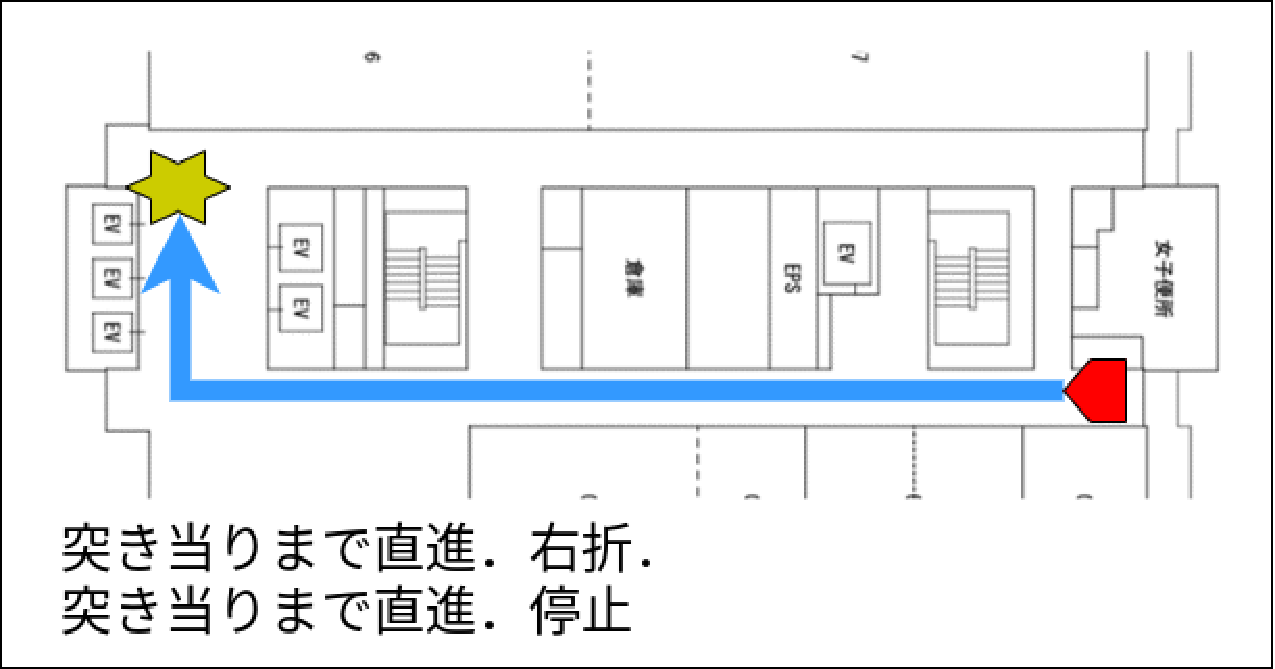
\includegraphics[keepaspectratio, width=57mm]{images/pdf/scenario/scenario05.pdf}
            \subcaption{Scenario 05}
            \label{image1}
        \end{minipage} &
        \begin{minipage}[t]{0.5\textwidth}
            \centering
            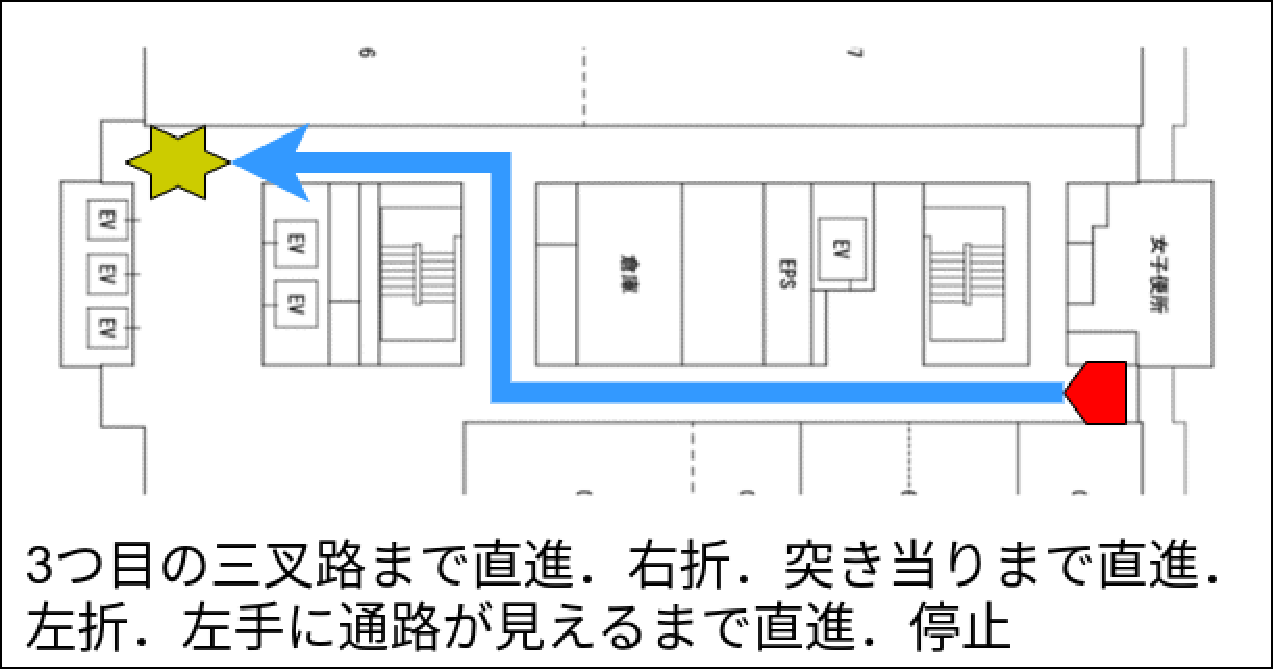
\includegraphics[keepaspectratio, width=57mm]{images/pdf/scenario/scenario06.pdf}
            \subcaption{Scenario 06}
            \label{fig:scenario24}
        \end{minipage}\\
        \begin{minipage}[t]{0.5\textwidth}
            \centering
            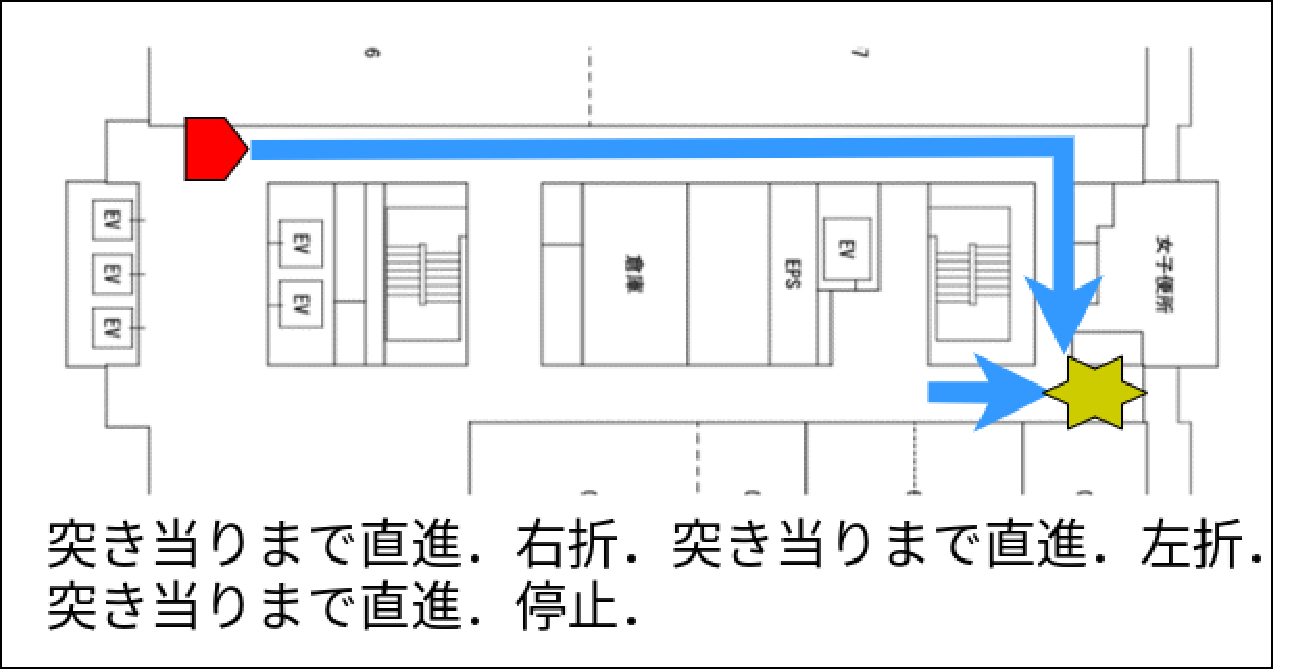
\includegraphics[keepaspectratio, width=57mm]{images/pdf/scenario/scenario07.pdf}
            \subcaption{Scenario 07}
            \label{imagess}
        \end{minipage}
    \end{tabular}
    \caption{Scenarios used in the experiment (Quoted from \cite{haruyama2023})}\label{fig:scenario_exp}
\end{figure*}

\begin{figure}[htbp]
    \centering
     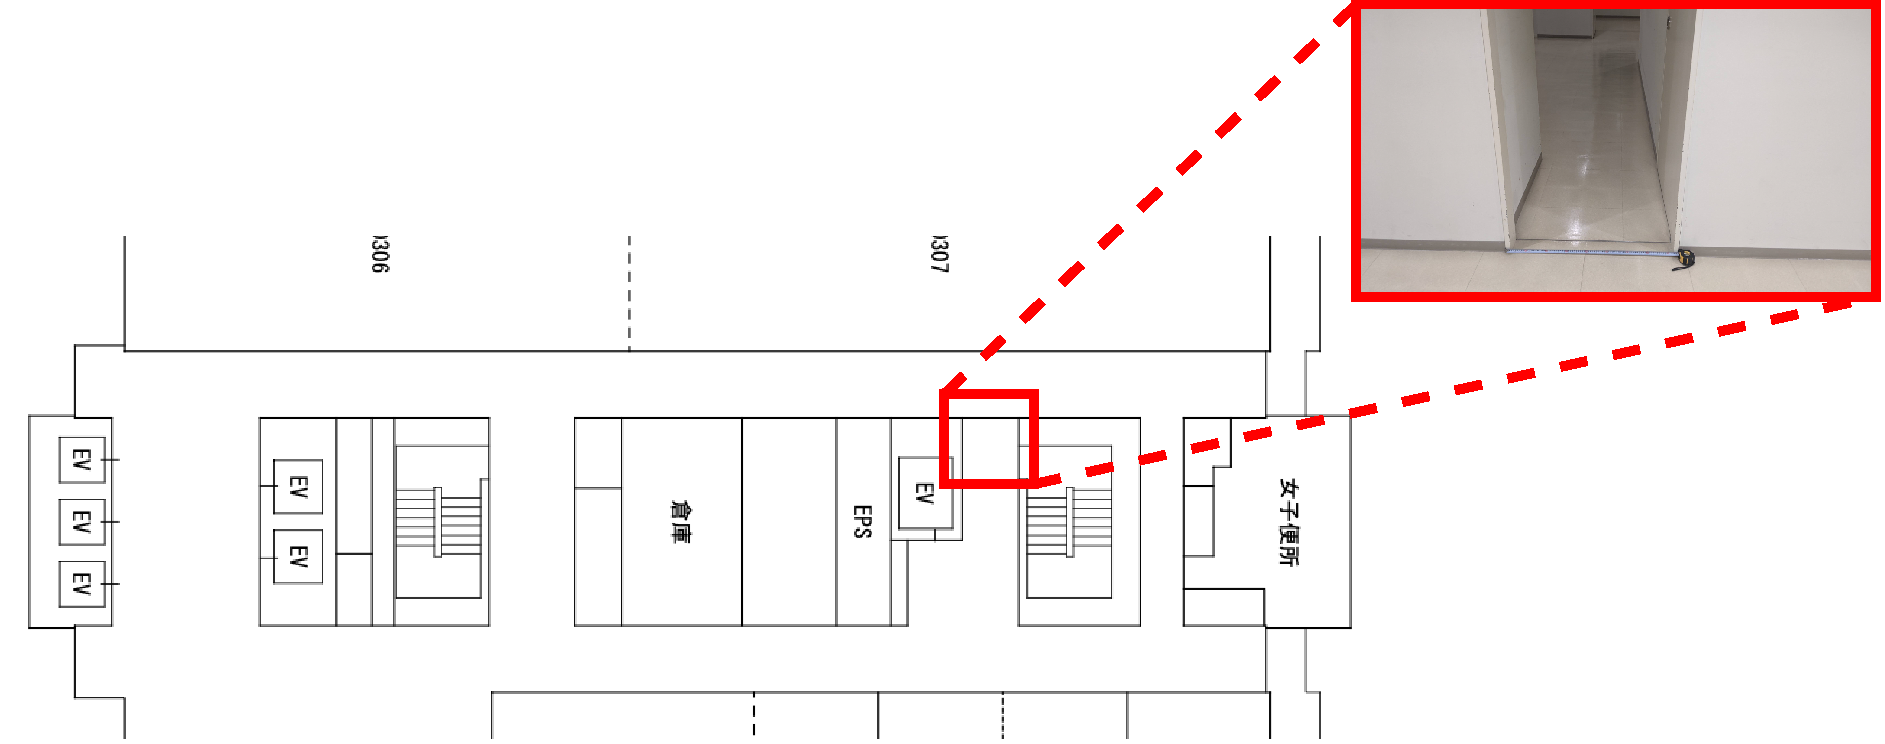
\includegraphics[width=130mm]{images/pdf/sce_semai.pdf}
     \caption{Example of narrow passage in experimental environment}\label{fig:semai}
\end{figure}

\clearpage
\subsubsection{通路追従モジュールの訓練}
まずはじめに通路分類モジュールの訓練を行う.
前述の経路をメトリックマップに基づいたルールベース制御器の出力を用いて,
3周し,データセットを収集する.
収集したデータは,1,2周目を訓練データとし,
3周目をテストデータとする.それぞれのデータ数は,
訓練データ5781,テストデータ2902であり.2つのデータ内のクラス間のデータ数は\tabref{tab:dataset}である.
訓練は損失関数の重みを\tabref{tab:cost},バッチサイズを32として,30epoch行った.

訓練後,テストデータに対する通路分類モジュールの正解率{(Accuracy)},適合率{(Precision)}を計算する.
\begin{table}[htbp]
    \centering
    \caption{Number of classes in the dataset}\label{tab:dataset}
    \begin{tabular}{c|c|c}
    \hline
    Class & Learning data &Test data        \\
    \hline
    直進   & 2760 & 1377\\
    突き当たり   & 90 & 45 \\
    角(右) & 549 & 279 \\
    角(左)& 567 & 288 \\
    十字路 & 0 & 0 \\
    三叉路(右)& 753 & 387 \\
    三叉路(中央)& 306 & 153 \\
    三叉路(左) & 747 & 369 \\
    \hline
    \end{tabular}
\end{table}

\begin{table}[htbp]
    \centering
    \caption{The weights assigned to each class in the experiment}\label{tab:cost}
    \begin{tabular}{c|c}
    \hline
    Class & Class weights         \\
    \hline
    直進   & 1\\
    突き当たり   & 5\\
    角(右) & 5\\
    角(左)& 5 \\
    十字路 & 1  \\
    三叉路(右)& 5  \\
    三叉路(中央)& 10  \\
    三叉路(左) & 5  \\
    \hline
    \end{tabular}
\end{table}
\subsubsection{経路追従モジュールの訓練}
次に経路追従モジュールの訓練を行う.
通路分類モジュールの訓練と同様の経路を,
オンラインで 模倣学習しながら1周走行する.
その際のステップ数は12000であった.

2つのモジュールを訓練後,シナリオを1例ずつ入力して,
ロボットの挙動を観察する.実験では,ロボットをシナリオの
スタート地点に移動して,自律移動を開始する.

\vspace{5zh}



\newpage
\subsection{実験結果}
テストデータに対する,通路分類モジュールの正解率と適合率を\tabref{tab:result}に示す.
この計算にはモデル評価用ライブラリである
torcheval\cite{torcheval}を用いた.
\begin{table}[htbp]
    \centering
    \caption{Evaluation results of the corridor classification module on test data.}
    \label{tab:result}
    \begin{tabular}{c|c}
    \hline
    Metrics & Value       \\
    \hline
    Accuracy   & 0.98 \\
    Precision   & 0.98 \\
    \hline
    \end{tabular}
\end{table}
% \begin{table}[]
%     \centering
%     \caption{intersection あーだのコーダの}\label{tab:acc}
%     \begin{tabular}{|c|c|}
%     \hline
%     指標 & 値
%     \hline
%     accuraty & 0.98 \\
%     適合率 & 0.4 \\
%     \hline
%     \end{tabular}
% \end{table}
% \newpage

\figref{fig:exp_path}に\figref{fig:scenario21}のシナリオを入力した実験の様子を示す.
キャプションは実行中の部分シナリオと,ロボットが現在位置する通路の特徴である.
図に示すように入力されたシナリオの道順に従い, 三叉路などの分岐路
で適切に経路を選択して自律移動する様子が見られた.
結果として,7例すべてでロボットが, 目的地へ到達した.
以上の結果から, 構築したカメラ画像とシナリオに基づいて, 
経路を追従して目的地まで自律移動するシステムの有効性が確認された.

\begin{figure*}[htbp]
    \begin{tabular}{ccc}
        \begin{minipage}[t]{0.5\textwidth}
            \centering
            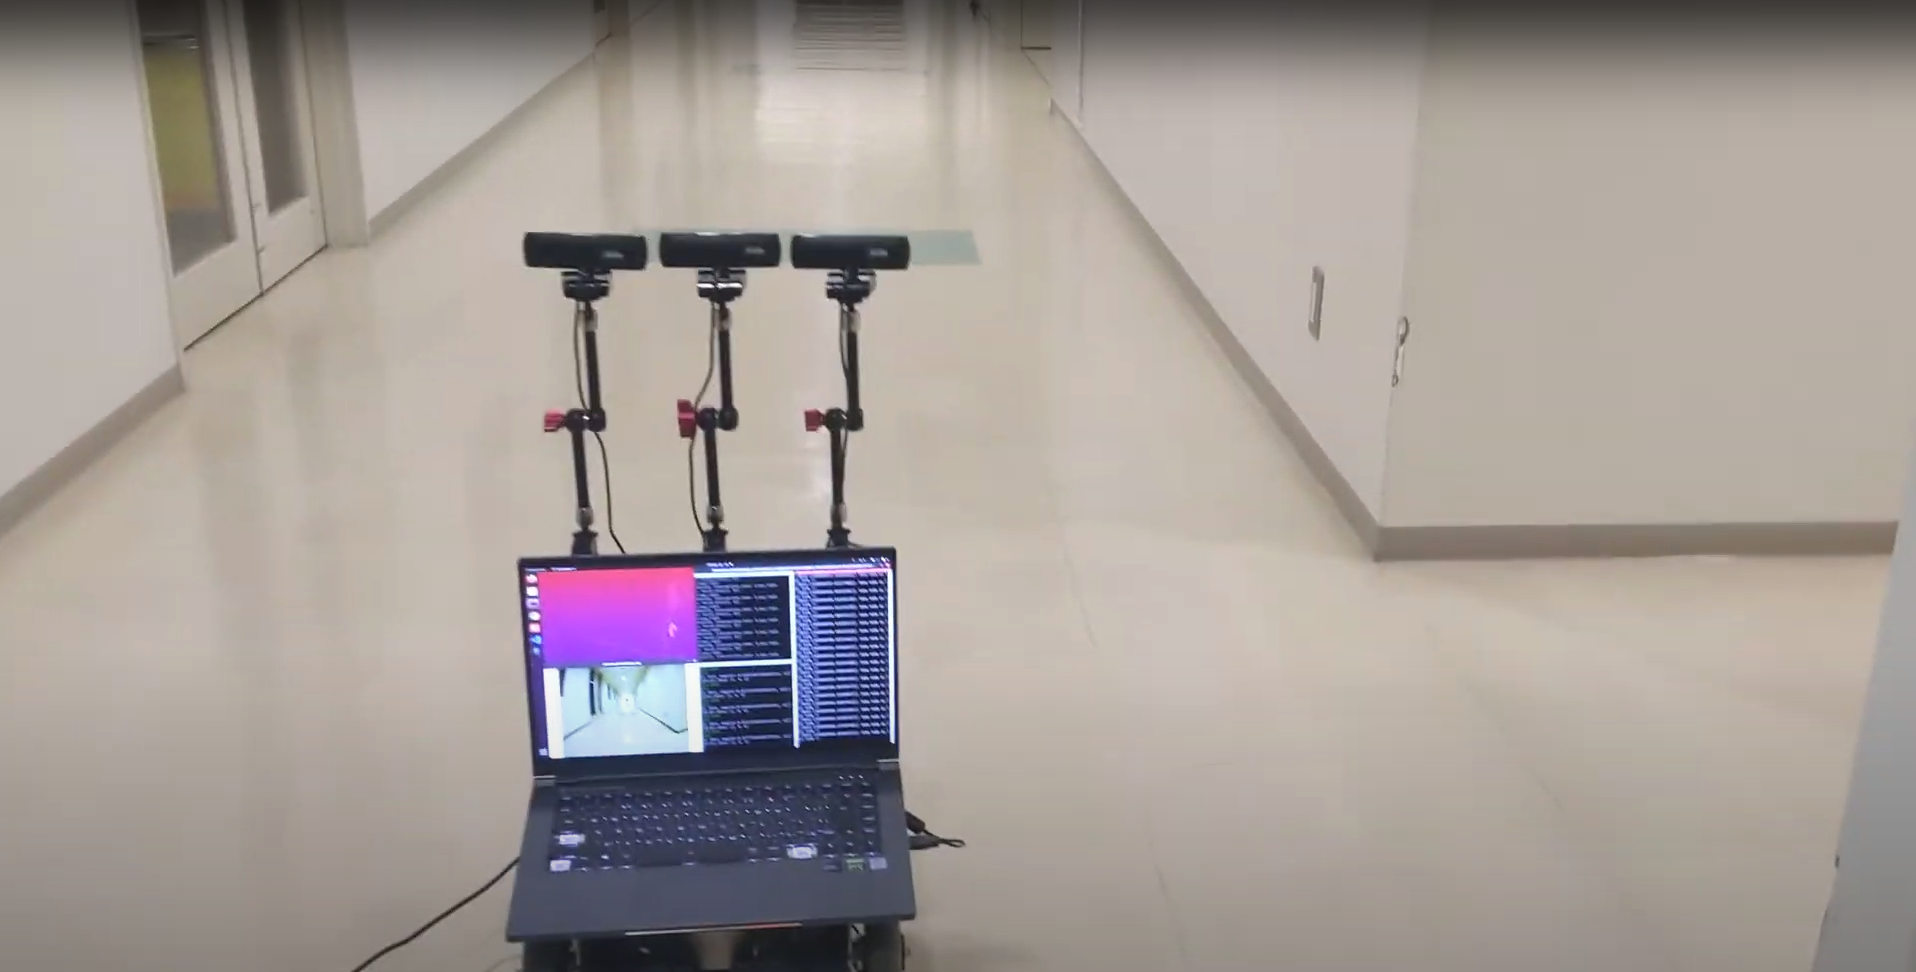
\includegraphics[keepaspectratio, width=70mm]{images/exp_path_follow_0.png}
            \subcaption{3つ目の三叉路まで直進(First 3-way)}
        \end{minipage} &
        \begin{minipage}[t]{0.5\textwidth}
            \centering
            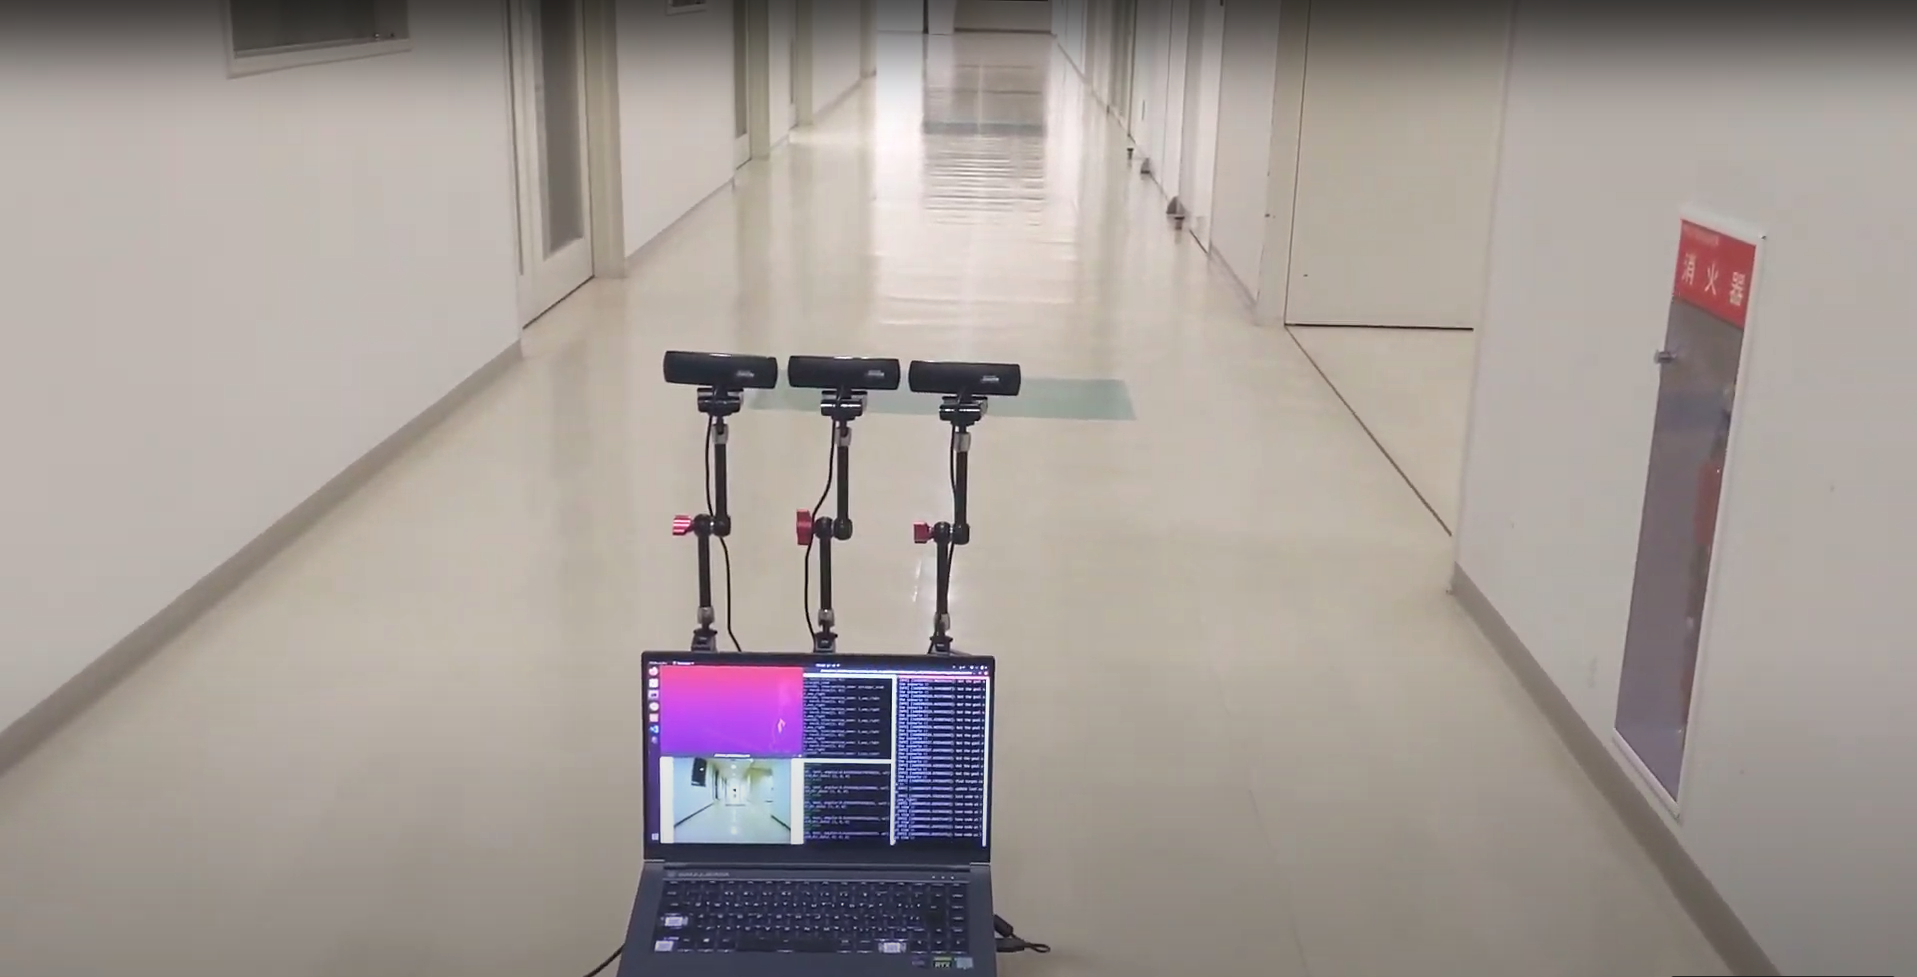
\includegraphics[keepaspectratio, width=70mm]{images/exp_path_follow_1.png}
            \subcaption{3つ目の三叉路まで直進(Second 3-way)}
        \end{minipage} \\

        \begin{minipage}[t]{0.5\textwidth}
            \centering
            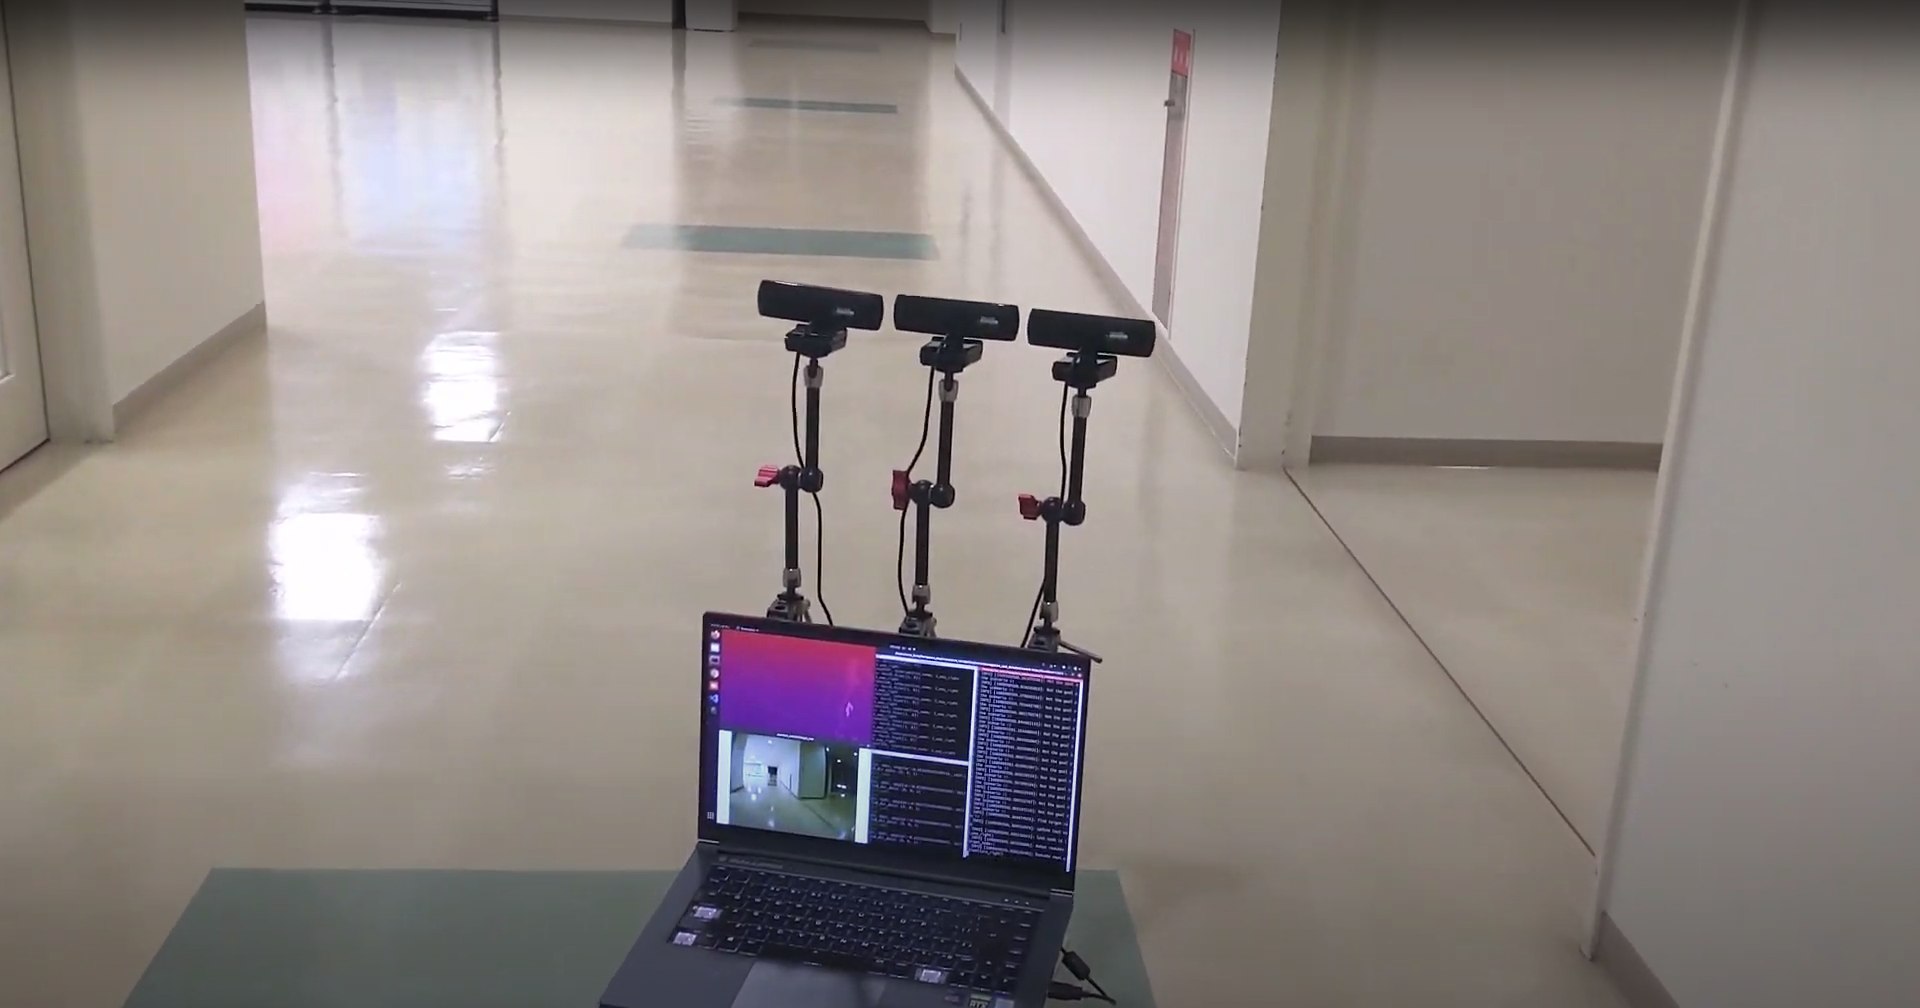
\includegraphics[keepaspectratio, width=70mm]{images/exp_path_follow_2.png}
            \subcaption{右折(Third 3-way)}
        \end{minipage} &
        \begin{minipage}[t]{0.5\textwidth}
            \centering
            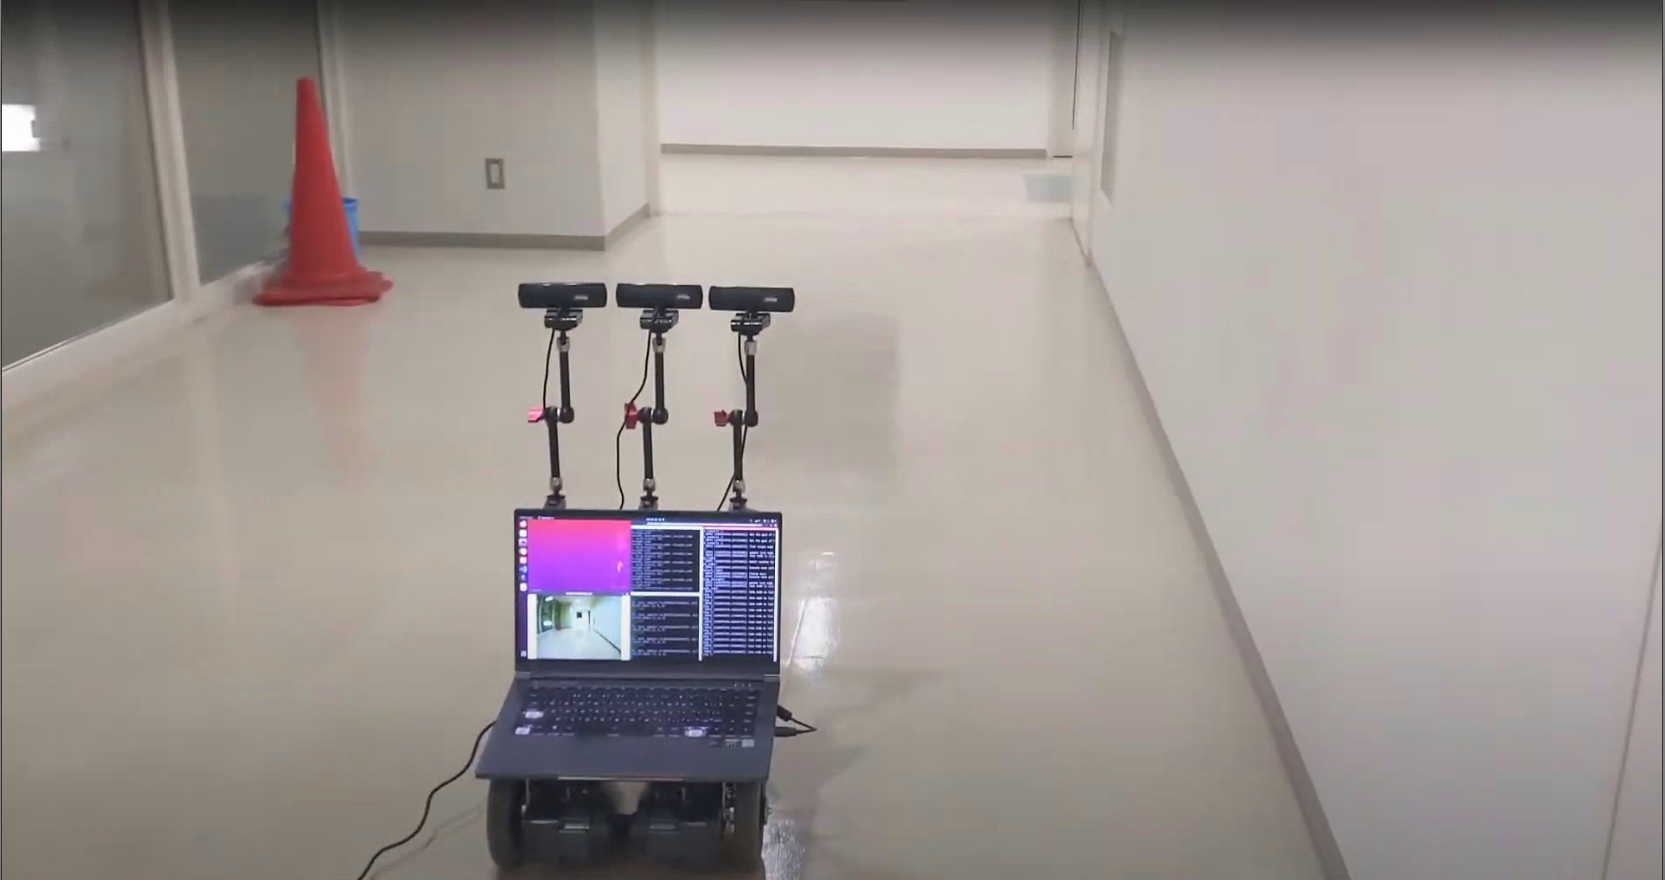
\includegraphics[keepaspectratio, width=70mm]{images/exp_path_follow_4.png}
            \subcaption{突き当たりまで直進(Straight road)}
        \end{minipage} \\
        \begin{minipage}[t]{0.5\textwidth}
            \centering
            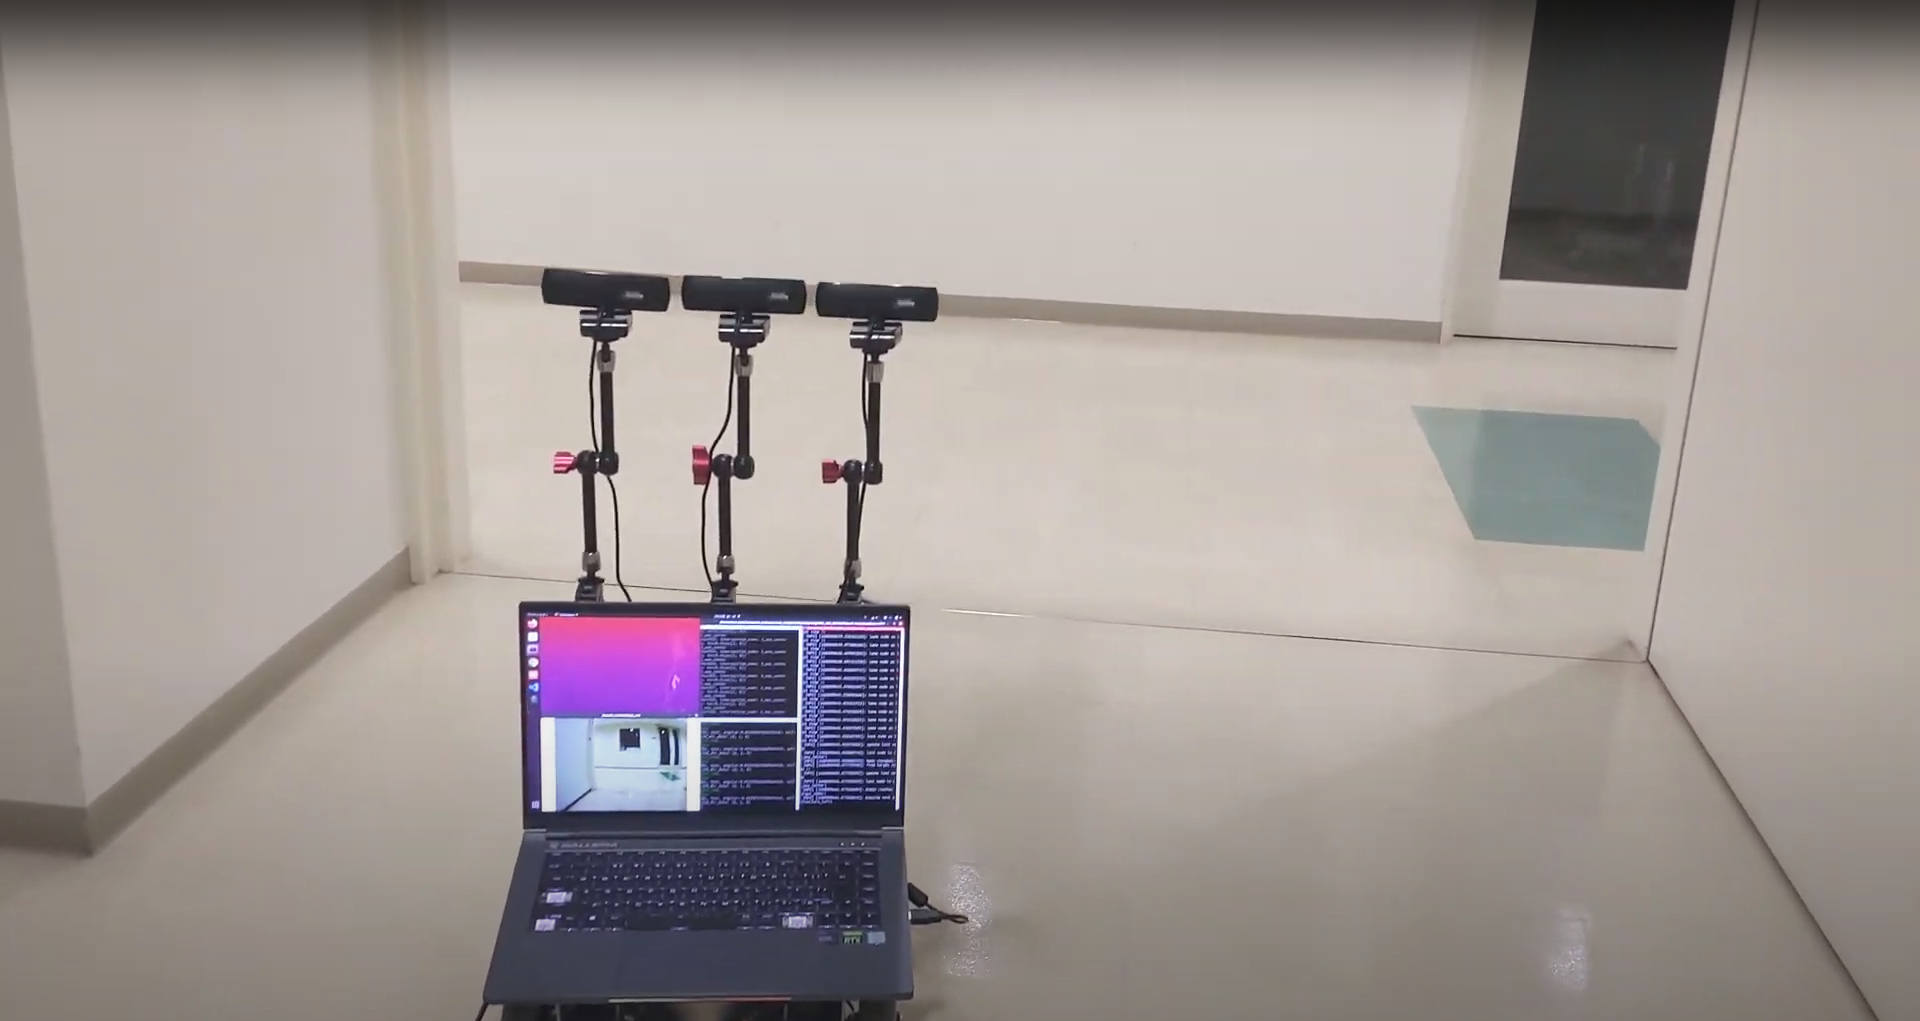
\includegraphics[keepaspectratio, width=70mm]{images/exp_path_follow_5.png}
            \subcaption{左折(End)}
        \end{minipage} &
        \begin{minipage}[t]{0.5\textwidth}
            \centering
            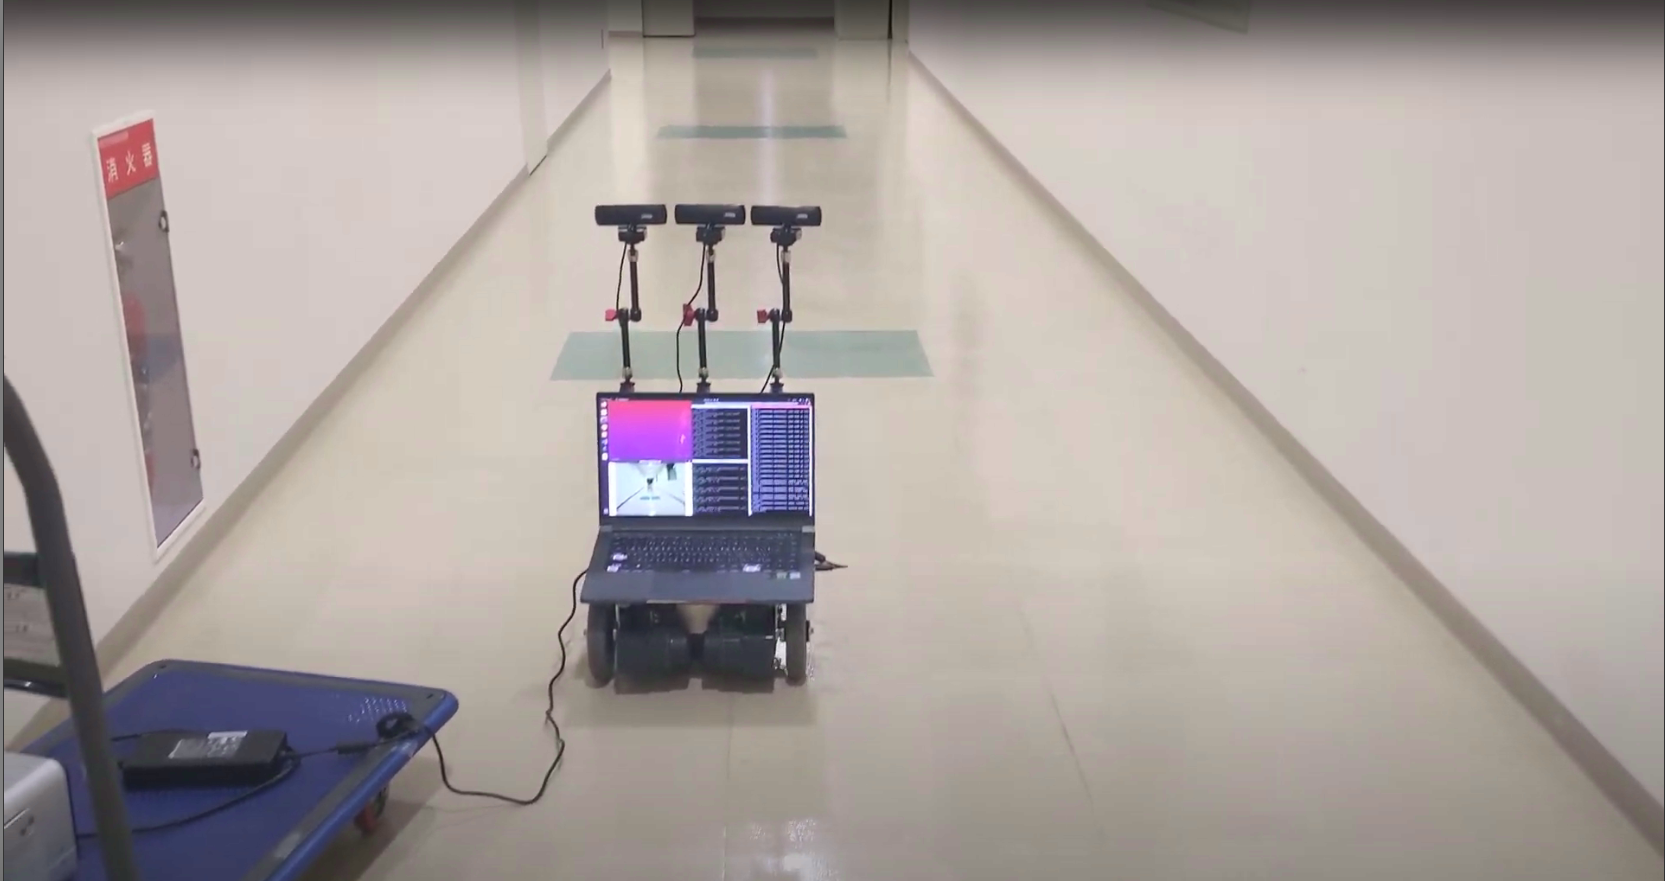
\includegraphics[keepaspectratio, width=70mm]{images/exp_path_follow_6.png}
            \subcaption{突き当たりまで直進(Straight road)}
        \end{minipage} \\
        \begin{minipage}[t]{0.5\textwidth}
            \centering
            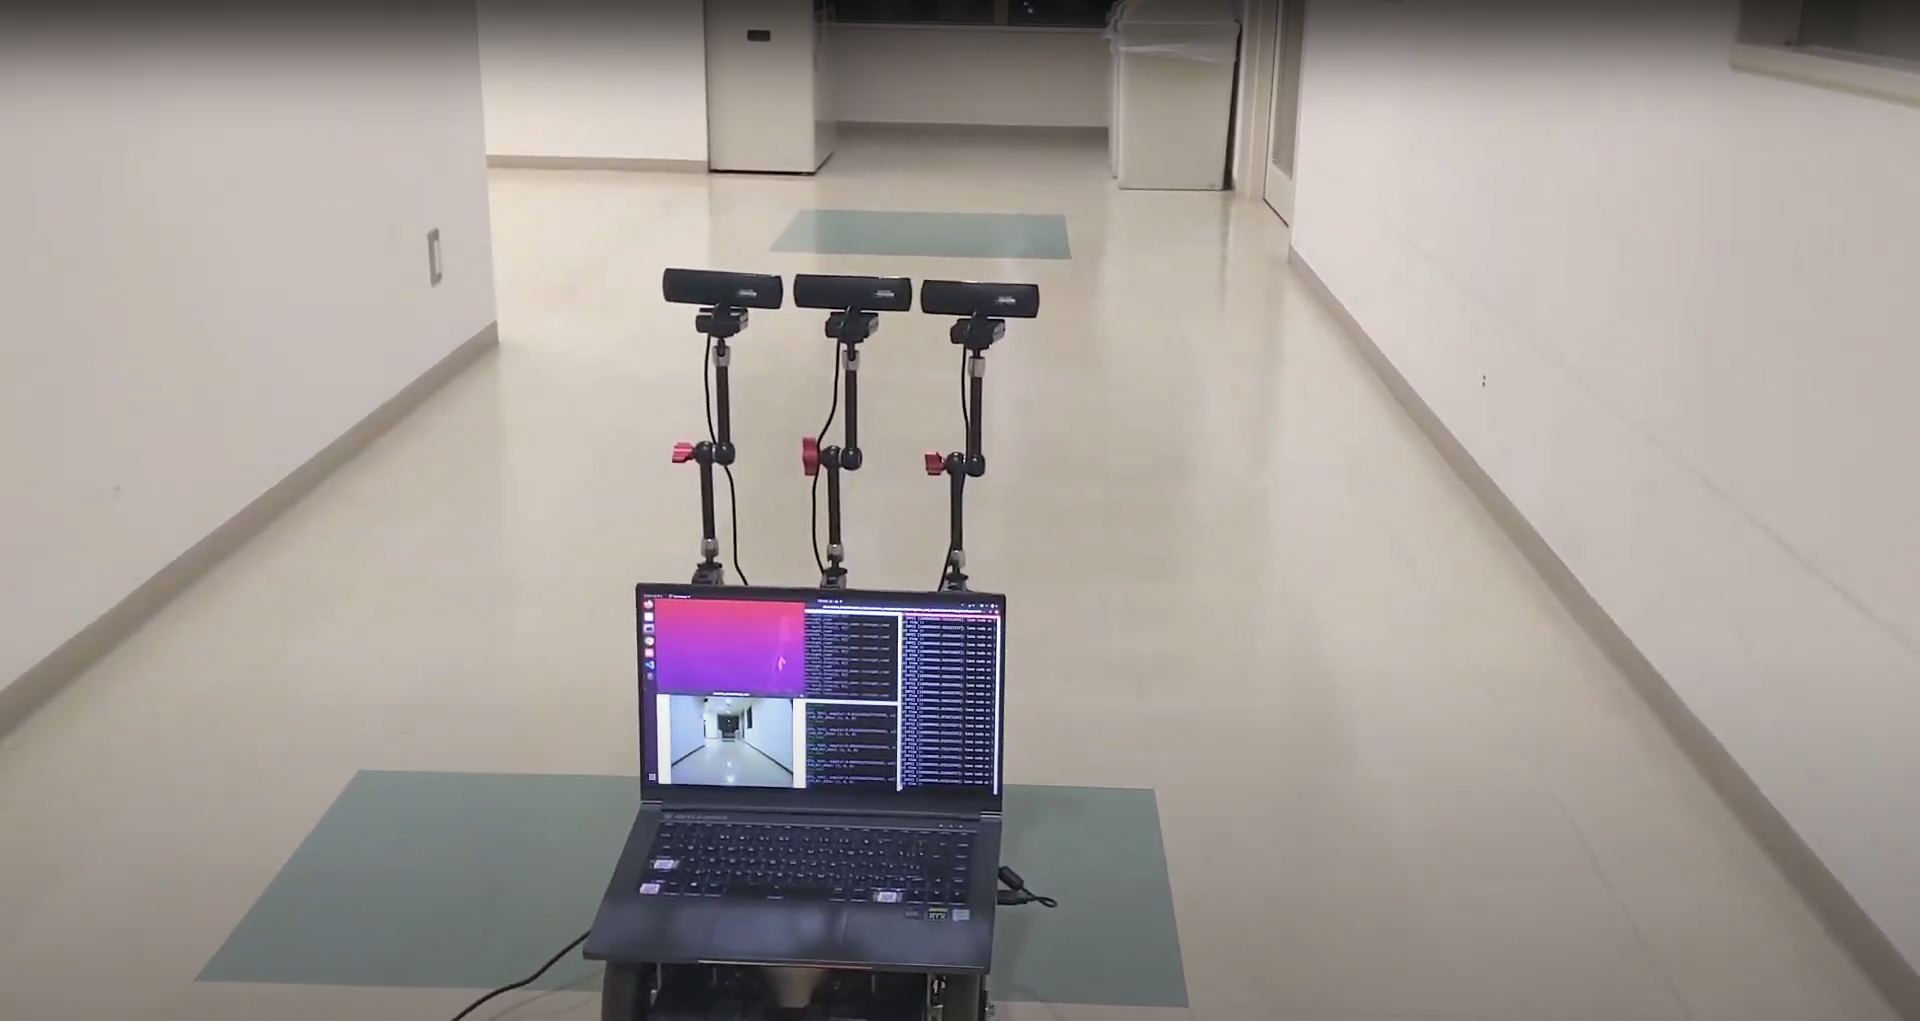
\includegraphics[keepaspectratio, width=70mm]{images/exp_path_follow_7.png}
            \subcaption{停止(End)}
        \end{minipage}
    \end{tabular}

    \caption{An example of the robot applied the constructed system (Quoted from \cite{haruyama2023})}\label{fig:exp_path}
\end{figure*}